\documentclass{article}

%\setlength{\parindent}{0cm}
%\setlength{\parskip}{\baselineskip}

\usepackage{bbm}
\usepackage{amsmath,amsthm,amssymb}
\usepackage{frcursive}
\usepackage{array}
\usepackage{hyperref} 
\usepackage{tikz}

\usetikzlibrary{positioning}
\tikzstyle{highlight}=[draw=gray,fill=black,text=white]
\newcommand{\ite}[3]{(#1 ~\tikz[baseline] \draw[->, -stealth] (0ex,.5ex)--(2ex,.5ex);~ #2 , #3)}


\newcommand{\comment}[1]{}

\newcommand{\Z}{\mathbbm{Z}}
\newcommand{\R}{\mathbbm{R}}
\newcommand{\N}{\mathbbm{N}}
\newcommand{\Q}{\mathbbm{Q}}
\newcommand{\C}{\mathbbm{C}}
\newcommand{\imu}{\text{\textcursive{i}}}
\newcommand{\eul}{\text{\textcursive{e}}}
\newcommand{\ele}{\mathrm{e}}
\newcommand{\qu}{\mathrm{q}}
\newcommand{\re}{\mathrm{r}}
\newcommand{\supp}{\mathrm{supp}}
\newcommand{\dom}{\mathrm{dom}}
\newcommand{\cod}{\mathrm{cod}}

\theoremstyle{theorem}
\newtheorem{theorem}{Theorem}
\newtheorem*{corollary}{Corollary}
\newtheorem{proposition}{Proposition}
\newtheorem{lemma}{Lemma}

\theoremstyle{definition}
\newtheorem*{definition}{Definition}
\newtheorem*{remark}{Remark}

\theoremstyle{definition}
\newtheorem{example}{Example}[section]

\begin{document}
\title{Efficiently representing the integer factorization problem using binary decision diagrams}
\author{David Skidmore}
\date{29 April 2017}
\maketitle

\begin{abstract}
\noindent Let $p$ be a prime positive integer and let $\alpha$ be a positive integer greater than $1$. A method is given to reduce the problem of finding a nontrivial factorization of $\alpha$ to the problem of finding a solution to a system of modulo $p$ polynomial congruences where each variable in the system is constrained to the set $\{0,\dots,p-1\}$. In the case that $p=2$ it is shown that each polynomial in the system can be represented by an ordered binary decision diagram with size less than 
$$20.25 \log_2(\alpha)^3 + 16.5 \log_2(\alpha)^2 + 6\log_2(\alpha)$$
whereas previous work on the subject has only produced systems in which at least one of the polynomials has an ordered binary decision diagram representation with size exponential in $\log_2(\alpha)$.

Using a different approach based on the Chinese remainder theorem we prove that for $\alpha \geq 4$ there is an alternative system of boolean equations whose solutions correspond to nontrivial factorizations of $\alpha$ such that there exists a $C>0$, independent of $\alpha$, such that for any order $\sigma$ on the variables in the system every function in the system can be represented by a $\sigma$-OBDD with size less than 
$$C\log_2(\log_2(\alpha))^2 \log_2(\alpha)^{4}.$$
\end{abstract}

\newpage

\tableofcontents

\newpage

\section{Introduction}
For all positive integers $x$ and $p$ with $p$ prime, $x$ can be uniquely written in the form
$$\sum_{n=0}^{m}x_np^n$$
where $m \in \N_0 = \{0,1,\dots\}$, $x_m \neq 0$, and each $x_n \in \{0,\dots, p-1\}$. This summation is called the \textit{base $p$ expansion of $x$}. 

If $p \in \N=\{1,2,\dots\}$ is prime then the base $p$ expansions of the positive integers can be extended to a field containing the rational numbers: $\Q_p$, the field of $p$-adic numbers. For every $x \in \Q_p$, there exists an $m \in \Z$ and a sequence $(x_n)_{n=m}^{\infty} : \{m,m+1,\dots\} \to \{0,1,\dots,p-1\}$, $n \mapsto x_n$ such that
$$x = \sum_{n=m}^{\infty}x_np^n.$$
We call the sum in the preceding equality the \textit{$p$-adic expansion of $x$}. If $x \in \N$ then $x$ has $p$-adic expansion $x_0+x_1p+\dots + x_mp^m+0p^{m+1}+0p^{m+2}+0p^{m+3}+\dots$ (for $k>m$ the coefficient of $p^k$ is zero) where $x_0+x_1p+\dots+x_m p^m$ is the base $p$ expansion of $x$.

For each $x \in \Q_p$ and $n \in \Z$ the \textit{$n$th $p$-adic digit of $x$} is defined to be the coefficient of $p^n$ in the $p$-adic expansion of $x$. If $x \in \Q_p$ is such that for all $n \in \Z$ the $n$th $p$-adic digit of $x$ is $0$ whenever $n<0$ then $x$ is called a \textit{$p$-adic integer}. The collection of all $p$-adic integers is denoted by $\Z_p$ and forms a subring of $\Q_p$. 

In this document we are primarily concerned with two related issues. First, for any prime $p$, representing the arithmetic operations of addition, multiplication, subtraction, and division on $\Z_p$ as a sequence of multivariate polynomials in the $p$-adic digits of their arguments. Second, the reduction of the integer factorization problem (FACT) to the problem of solving a system of polynomial equations. 

\subsection{Previous Work}
In recent years there have been several studies concerned with both the reduction of FACT to the Boolean satisfiability problem (SAT) and the performance of (modern day) SAT solvers in finding a solution to the resulting reduction, \cite{Asketorp, Eriksson, Forsblom}. All of these studies performed the reduction using recursive algorithms obtained from modeling digital adder and multiplier circuits using a Boolean algebra. The SAT solvers applied to the resulting reductions were general purpose, rather than being designed for the specific problem of FACT. 

Conjunctive Normal Form (CNF) is a particular type of normal form for mathematical expressions representing elements of a Boolean algebra \cite{Gomes}. According to Gomes and others, CNF has a number of desirable characteristics which has lead to it becoming the generally accepted input format for modern SAT solvers \cite{Gomes}. As such, previous studies concerning FACT to SAT reduction have made it a point that their algorithms produce output in CNF format. 

The relevance of this to the current paper is that the reductions performed in aforementioned FACT to SAT studies were equivalent to reducing FACT to a system of polynomials with coefficients taken from the prime field with two elements. Similarly, due to the fact that multi-valued logic functions can be represented by polynomials over finite fields \cite{Carnielli2, Stankovic}, converting FACT to a system of polynomials over a finite field of prime order greater than two is equivalent to reducing FACT to a multivalued logic satisfiability problem (MV-SAT). 

A \texit{Boolean ring} is a commutative ring with identity in which every element is idempotent, i.e. every $x$ in the ring satisfies $x^2=x$. Every Boolean ring is equivalent to a Boolean algebra. Using a Boolean ring, in \cite{Lomonaco}, Samuel J. Lomonaco created FACT to SAT reduction algorithms with output in both Algebraic Normal Form (ANF) and Disjunctive Normal Form (DNF), rather than in CNF, and corresponding integer factorization algorithms that do not rely on general purpose SAT solvers. Additionally, Lomonaco gave representations of arithmetic operations in terms of polynomials defined by recurrence relations inspired by common arithmetic algorithms, such as the standard algorithm for multiplication, also called long multiplication. The work done by Lomonaco on the reduction of FACT to DNF SAT was further studied and expanded on by S. Bagde \cite{Bagd/2013}.

Both the studies utilizing CNF and those using ANF and DNF concluded that their algorithms were far inferior to commonly used specialized FACT algorithms such as the general number field sieve. 

The following definitions, provided by Liska et al., can be found in \cite{Liska}. They represent performance measures of algorithms.

\begin{definition}
\textit{Expression Swell} is a common phenomenon of exact computations in which the size of numbers and expressions involved in a calculation grows dramatically as the calculation progresses.
\end{definition}

\begin{definition}
\textit{Intermediate Expression Swell} is an important special case of expression swell in which, during the middle stages of a calculation, intermediate expressions can expand substantially, but the final results of the calculation are comparatively simple.
\end{definition}

As an example of expression swell, interpret the following two expressions, in indeterminates $X = \{x_1, x_2, x_3, x_4, x_5, x_6\}$, as sequential states of a calculation, with the first line representing the initial state and the second line the final state.
\begin{align*}
(x_1+x_2) (x_3+x_4) (x_5+x_6) \\
x_1 x_3 x_5 + x_1 x_3 x_6 + x_1 x_4 x_5 + x_1 x_4 x_6 + x_2 x_3 x_5 + x_2 x_3 x_6 + x_2 x_4 x_5 + x_2 x_4 x_6
\end{align}
The first state of the calculation, considered as a term, contains 3 additions and 2 multiplications while the second contains 7 additions and 16 multiplications. Using Polish notation, the first expression is equivalent to a string consisting of 11 characters taken from the set $X \cup \{{+},\times\}$, i.e. $\times \times {+} x_1 x_2 {+} x_3 x_4 {+} x_5 x_6$. However, using the same set of characters, the second expression is equivalent to a string consisting of 47 characters.

As an example of intermediate expression swell, interpret the following as sequential states of a calculation with the first line being the initial state and the third line being the final state.
\begin{align*}
(0+0) (0+0) (0+0) \\
0 0 0 + 0 0 0 + 0 0 0 + 0 0 0 + 0 0 0 + 0 0 0 + 0 0 0 + 0 0 0 \\
0
\end{align}

Generally speaking, expression swell can lead to an exponential increase in the sizes or numbers of expressions involved in a calculation. Therefore it is not surprising that, in computer algebra, expression swell can lead to significant increases in both the memory needed and CPU time required by a computer to perform a given calculation. 

In many cases converting a propositional expression to a particular normal form such as CNF can lead to significant expression swell, either in the intermediate stages of the conversion or in the final output. Previous studies have only utilized recursive algorithms inspired by existing arithmetic algorithms to generate an initial set of expressions which is then converted to the desired normal form. The initial expressions resulting from these algorithms exhibit a deeply nested structure not conducive to conversion. This suggests that expression swell had a major impact on the efficiency of the algorithms used in the previously mentioned studies.

A \textit{boolean function} is a $\{0,1\}$-valued function in a finite number of $\{0,1\}$-valued (\textit{boolean}) variables. 
\begin{example}
The binary operation $\oplus : \{0,1\} \times \{0,1\} \to \{0,1\}$ (exclusive disjunction, boolean XOR, modulo-$2$ addition) is defined by
$$x \oplus y = \begin{cases} 0 \textrm{ if } x = y \\ 1 \textrm{ if } x \neq y \end{cases}.$$
\end{example}
Every boolean function can be represented as a \textit{boolean polynomial}: a polynomial with coefficients taken from $\{0,1\}$, with addition replaced by modulo-$2$ addition, and which is of degree at most $1$ for any particular variable. Equivalently, a boolean polynomial can be thought of as a typical polynomial with integer coefficients interpreted over the integers mod $2$, e.g. $(f \mod{2})$ where $f$ is a polynomial with integer coefficients.

Let $\alpha$ be a positive integer greater than $1$ with binary expansion 
$$\alpha_0 + 2\alpha_1 + \dots + 2^{\beta-1}\alpha_{\beta-1}$$
where $\beta-1 = \lfloor \log_2(\alpha) \rfloor$ and for every real number $t$, $\lfloor t \rfloor$ represents the largest integer $u$ such that $u \leq t$. For each nonnegative integer $m$ let $f_m : \{0,1\}^{2\beta} \to \{0,1\}$ be the boolean function such that $f_m(x_0,x_1,\dots,x_{\beta-1},y_0,y_1,\dots,y_{\beta-1})$ (represented by $f_m(\vec{x},\vec{y})$) gives the the coefficient of $2^m$ in the binary expansion of the product
$$(x_0 + 2x_1 + \dots + 2^{\beta-1}x_{\beta-1})(y_0 + 2y_1 + \dots + 2^{\beta-1}y_{\beta-1}).$$
Every factorization of $\alpha$ corresponds to a solution to the system
\begin{align*}
\alpha_0 \oplus f_0(\vec{x},\vec{y}) &= 0  \\
\alpha_1 \oplus f_1(\vec{x},\vec{y}) &= 0  \\
 &\vdots \\
\alpha_{\beta-1} \oplus f_{\beta-1}(\vec{x},\vec{y}) &= 0 \\
f_{\beta}(\vec{x},\vec{y}) &= 0 \\
 &\vdots \\
f_{2\beta-1}(\vec{x},\vec{y}) &= 0 .
\end{align}
Let $S_{\alpha}$ denote the set of polynomials $\{\alpha_m \oplus f_m \mid m \in \N_0\}$ where $f_m = f_m(\vec{x},\vec{y})$, if $m\geq \beta$ then $\alpha_m = 0$, and if $m \geq 2\beta$ then $f_m = 0$. We'll refer to $S_{\alpha}$ as the \textit{standard representation}.

A \textit{boolean circuit} is a directed acyclic graph with all nodes labeled by elements of a finite set. The labels consist of constants from $\{0,1\}$, variables, and operators, typically $\land$, $\lor$, and $\oplus$. Nodes labeled by constants or variables have an in-degree, also called \textit{fan-in}, of $0$ and any such node is referred to as an \textit{input node}. A node with out-degree, also called \textit{fan-out}, $0$ is an \textit{output node}. Any node with in-degree strictly greater than $0$ is called a \textit{gate} and is labeled by an operator. Without loss of generality we will assume that every gate label corresponds to a binary operator and that every node labeled with such an operator has in-degree of exactly $2$. If $C$ is a circuit with $n$ variable labels we will say that $C$ is a \textit{circuit in $n$ variables}.

The \textit{size} of a boolean circuit is its number of gates. The \textit{depth} of a circuit is the length of one of its longest paths.

A \textit{boolean formula} is a boolean circuit where all nodes have an out-degree of at most $1$. Boolean formulae may be thought of as a notationally independent way of representing mathematical terms corresponding to boolean functions.

All previous work on the subject of representing integer factorization as a system of boolean polynomials proceeds via finding different ways to represent the elements of $S_{\alpha}$. This is usually done by way of taking a boolean circuit representing a binary multiplier and then representing that circuit as a collection of single output boolean formulae the $m$th such formula corresponding to $f_m$, these formulae are then equated to the binary digits of $\alpha$ giving the equations $f_m = \alpha_m$ or equivalently $\alpha_m \oplus f_m = 0$. We note that typically each $\alpha_m \oplus f_m = 0$ is replaced by $1 \oplus \alpha_m \oplus f_m = 1$ as most previous work tends to use boolean algebras rather than boolean rings.

If the goal is simply to represent FACT as an instance of CNF SAT then it is already known that this can be done efficiently using the Tseitin transformation on a multiplier circuit to produce a $3$-SAT instance with size linear in the size of the input circuit \cite{KrSt/2016}. For a pair of $n$-bit numbers there are multiplier circuits with size $\mathcal{O}(n \log_2(n) \log_2(\log_2(n))$ \cite{Wege/1991} so the boolean formula resulting from the transformation is not very large. The result of the Tseitin transformation is not equivalent to the original formula, it is equisatisfiable. For our intents and purposes two boolean formulae corresponding to boolean functions $f$ and $g$ are equisatisfiable if and only if the equations $f=1$ and $g=1$ either both have a solution or neither have a solution. By comparison the two formulae are equivalent if and only if the equation $f=1$ has the same solution set as $g=1$. For example, in the boolean variables $x$ and $y$, $f=x \oplus y$ is equisatisfiable, but not equivalent, to $g=xy$ since $x=1,y=0$ is a satisfying assignment for $f$ but not $g$ and $x=1,y=1$ is a satisfying assignment for $g$. Furthermore 3-SAT is NP-complete and all attempts to solve the SAT problem resulting from the application of the Tseitin transformation to a multiplier circuit have met with very little success regardless of what type of multiplier circuits have been used. 

Another problem with using $S_{\alpha}$ as the base for a reduction algorithm is that there is at least one boolean normal form for which it is infeasible to represent the elements of $S_{\alpha}$ when $\alpha$ is large: the representation of a boolean function by an \textit{ordered binary decision diagram} (OBDD), a special type of labeled rooted directed acyclic graph together with a total order on the labels of its nodes. In 2005 Philipp Woelfel showed that regardless of the linear order used, $f_{n-1}$ will have an OBDD representation with at least $2^{\lfloor n/2 \rfloor}/61-4$ nodes \cite{Woel/2005}.

It is also worth noting that in all of the previously mentioned studies a well known family of polynomials, the elementary symmetric polynomials, frequently appear. This fact was noted by Lomonaco but not explored.

\subsection{Problem Statement}
Before giving the problem statement it is necessary to introduce a bit of notation. For any set $T$, $(x_i)_{i \in T}$ is used to denote the function with domain $T$ which for all $i \in T$ maps $i$ to $x_i$. The codomain of such a function will be specified in context if relevant. In the case that $T$ is some finite product of totally ordered sets, we may opt to use a subscript superscript notation that mimics the indexing conventions of summations. For example, $(x_{i,j})_{i=1}^{2}_{j=0}^{i}$ has domain $\{ (u,v) \mid (u,v) \in \{1,2\} \times \{0,1,2\} \ , \ v \leq u \}$. Sequences (tuples) fall under this convention and so we emphasize here not to confuse sequence (tuple) evaluation with component-wise multiplication by a scalar. For example, if $x$ is a sequence, say $x=(x_i)_{i=1}^{\infty}$, then for any $k \in \N$, $x(k) = x_k$. Lastly, if $f$ is a function and $T$ is a set then $f \subseteq T$ means that the image of $f$ is contained in $T$ and $f \subset T$ means that the image of $f$ is contained in $T$ but not equal to $T$.

Let $p$ be a prime number. Every $x \in \Z_p$ can be associated with a unique sequence $(x_n)_{n=0}^{\infty} \subseteq \{0,\dots,p-1\}$ where for each $n \in \N_0$, $x_n$ is the $n$th $p$-adic digit of $x$; we call this sequence the \textit{$p$-adic digit vector associated with $x$}. 

We define the \textit{arithmetic operations on $\Z_p$} to be the collection $\{{}+{},\times,{}-{},/\}$ where $+$ and $\times$ represent the field operations of addition and multiplication restricted to $\Z_p$, $-$ represents the binary operation of subtraction restricted to $\Z_p$, and $/$ denotes the partial binary function of division restricted to the set of all $(x,y) \in \Z_p^2$ such that the $0$th p-adic digit of $y$ is nonzero. 

If $\star \in \{{}+{},\times, {}-{},/\}$ and $f = (f_n)_{n=0}^{\infty}$ is a sequence of integer valued polynomial functions, each defined for all pairs of $p$-adic digit vectors, then $f$ is called a \textit{sequence of polynomials associated with $\star$} if and only if for all $x,y \in \Z_p$ and $n \in \N_0$, if $x \star y$ is defined then
$$(x \vec{\star} y)(n) \equiv f_n(\vec{x},\vec{y}) \pmod{p} $$
where  $\vec{x}$, $\vec{y}$, and $x \vec{\star} y$ denote, respectively, the $p$-adic digit vectors associated with $x$, $y$, and $x \star y$.

We can now give the formal problem statements.
\begin{itemize}
\item For each arithmetic operation on $\Z_p$ can we obtain an associated sequence of polynomials using a method that is not based upon simulating arithmetic algorithms or digital adder and multiplier circuits?

\item How are the elementary symmetric polynomials related to the sequences of polynomials associated with the arithmetic operations on $\Z_p$?

\item In the case that $p=2$, given a positive integer $\alpha$ greater than $1$, can the problem of finding a nontrivial factorization of $\alpha$ be reduced to finding a solution to a system of boolean polynomial equations such that each polynomial in the system can be represented by an OBDD whose number of nodes is less than some fixed power of $\log_2(\alpha)$?
\end{itemize}

\subsection{Significance}
The questions asked in the problem statement are related to several important mathematical and computational problems, in particular the integer factorization problem.

Many cryptosystems in wide use today, such as RSA, are based on the presumed difficulty of integer factorization. The best known methods, such as the general number field sieve, are subexponential time algorithms; incapable of posing a threat to a system like RSA.

Secondly, the literature that is available on the subject is scarce and narrow in scope. This indicates that it may not have received as much research attention as it should have. For example, although previous studies have resulted in algorithms which appear to take time exponential in the logarithm of the number to be factored, nothing has been proven about their running times, with the conjectures about them based purely upon data gathered via computational experiments, that is to say by running the algorithms on a large amount of numbers and recording the running times. Another point to be made is that not very much has been said about the structure of the systems of equations representing the integer factorization problem resulting from the transformation methods used in previous studies. Part of the reason for this may be due to the fact that the majority of previous studies on the subject have relied on transformation algorithms that were based upon various recursions. This may have served to obfuscate any structure that was present in the results, or at the least present a viewpoint of said structure which may be particularly difficult for humans to analyze compared to the viewpoint that a different, chiefly non-recursive, approach may offer.

\subsection{Layout of Document}
The background information section serves as a reference for various pieces of background information utilized in this thesis. 

We first define quotient and remainder functions which are then used to obtain recurrence relations for sequences of polynomials associated with each arithmetic operation on $\Z_p$. Sets of such recurrence relations are available from previous work for $\Z_2$. 

A solution for each of the recurrence relations is presented. Bits and pieces of these solutions can be found in the literature, although not all in one place as far as the author is aware.

We show how the factorization of $\alpha$ can be expressed as a system of polynomials $S_{\alpha}$ obtained from the aforementioned recurrence relation solutions. A method of reducing this system to a new system of polynomials $T_{\alpha}$ is given. The reduction method used by the author and the resulting system of polynomials is novel as far as the author can find.

We prove that when $p=2$, the polynomials making up the system $T_{\alpha}$ can each be represented by an OBDD with at most 
$$20.25 \log_2(\alpha)^3 + 16.5 \log_2(\alpha)^2 + 6\log_2(\alpha)$$ 
nodes. We show that with the ordering used for each polynomial in the system, there is an ordering of the polynomials of the system $g_0,g_1,\dots$ such that for each $m \in \N_0$ there is an ordering such that the OBDD size of $g_m g_{m+1}$ using this ordering has size $\mathcal{O}(\log_2(\alpha)^6)$. Furthermore using a different approach based on the Chinese remainder theorem we prove that for $\alpha \geq 4$ there is an alternative system of boolean equations whose solutions correspond to nontrivial factorizations of $\alpha$ such that there exists a $C>0$, independent of $\alpha$, such that for any order $\vartriangleleft$ on the variables in the system every function in the system can be represented by an OBDD using the total order $\vartriangleleft$ with size less than $C\log_2(\log_2(\alpha))^2 \log_2(\alpha)^{4}$. This is a new result on the subject as far as the author can tell and important because the ordering of the variables in an OBDD can have a drastic effect on its size. That is to say, for large enough $n$, there is a function in $n$ variables which has one variable ordering for which the smallest OBDD has size polynomial in $n$ and has another variable ordering for which the smallest OBDD has size exponential in $n$.

Lastly we discuss a possible factorization algorithm utilizing the system $T_{\alpha}$ represented as a collection of OBBDs and discuss some open questions directions for future work.

\newpage

\section{Background Information}
\subsection{Polynomial Rings}
Before getting started, we need to introduce a small bit of notation. If $R$ is a ring then $0_R$ denotes the additive identity of $R$, and if $R$ is a ring with unity then $1_R$ denotes the multiplicative identity of $R$.

This section gives a quick introduction to polynomials as they are frequently used throughout this thesis informally with intended interpretation given by context. The elementary symmetric polynomials are also defined as they have appeared in previous research on the same subject as this thesis and are given a generalization within this thesis. More information can be found in \cite{lang}.

Let $R$ be a ring and let $X = \{x_1,\dots,x_m\}$ be a collection of $m$ distinct symbols disjoint from $R$. Let $R[X]$, equivalently $R[x_1,\dots,x_m]$, denote the set of all functions mapping $\N_0^m \to R$ with finite support. Define addition on $R[X]$ pointwise and define multiplication on $R[X]$ by
$$\forall f,g \in R[X] \ \forall i \in \N_0^m \ (fg)(i) = \sum_{\substack{j,k \in \N_0^m \\ j+k=i}}[f(j) g(k)]$$
It follows that $R[X]$ together with the above operations of addition and multiplication forms a ring. This ring is called the \textit{ring of polynomials in $m$ indeterminates $X$ with coefficients in $R$}.

There is a more common and convenient notation with which to represent the elements of $R[X]$ which we describe here.

Let $M$ denote the free commutative monoid generated by the set $X$; that is, $M$ is the set consisting of all equivalence classes of strings over $X$, where two strings are equivalent if and only if one is a permutation of the other, together with the binary operation of string concatenation on $M$.  Without loss of generality we assume that $1_M$ is a symbol disjoint from $X$ which we let denote the identity element of $M$. If $y \in M$ then we define $y^0 = 1_M$. If $y \in M$ and $n \in \N$ then we define $y^n = y^{n-1}y$. Let $x = (x_1,\dots,x_m)$ and for each $i=(i_1,\dots,i_m) \in \N_0^m$ let $x^i = x_1^{i_1} \dots x_m^{i_m}$. Using these conventions, each element of $M$ can be uniquely written in the form $x^i$ where $i \in \N_0^m$.

We will identify each pair consisting of an element of $R$ and an element of $M$ with an element of $R^{\N_0^m}$. Suppose that $a \in R$ and $y \in M$. Let $i \in \N_0^m$ be such that $y = x^i$. Let $ay$ and $ya$ both denote the function mapping $\N_0^m$ into $R$ defined by
$$j \mapsto \begin{cases} a & \impliedby i=j \\ 0_R & \impliedby i\neq j \end{cases}$$ 

It follows that any $f \in R[X]$ can be represented by an infinite formal sum
$$\sum_{i \in \N_0^m}a_ix^i$$
where for each $i = (i_1,\dots,i_m) \in \N_0^m$, $a_i \in R$ and $a_i=0$ for all but a finite number of $i$.

We observe the following notational conventions when working in $R[X]$: for all $a \in R$, and $i,j \in \N_0^m$
\begin{itemize}
\item $a1_M = a$
\item If $R$ has unity then for all $i \in \N_0^m$, $1_Rx^i = x^i$
\end{itemize}

In the context of $R[X]$, for each $i \in \N_0^m$, $x^i$ is called a \textit{monomial}. If $f \in R[X]$ and 
$$f = \sum_{i \in \N_0^m}a_ix^i$$
where each $a_i \in R$ then for each $i \in \N_0^m$, $a_i$ is called the \textit{coefficient} of $x^i$ in $f$.

If $R$ does not have unity, then $R$ may be embedded in a ring with unity having the same characteristic as $R$. Therefore, unless stated otherwise, whenever working within a polynomial ring $R[X]$ we will assume that $R$ has unity, and thus so too does $R[X]$.

The map $R \to R[X]$ defined by $r \mapsto rx^0$ is a monomorphism of rings. We identify $R$ with its image under this map and so consider $R$ a subring of $R[X]$. Similarly, if $X'=\{x_{i_1},\dots,x_{i_l}\} \subseteq X$ has $l$ elements then $R[X']$ embeds into $R[X]$ under the ring monomorphism $R[X'] \mapsto R[X]$ which satisfies $ax_{i_1}^{j_1}\dots x_{i_l}^{j_l} \mapsto ax_{i_1}^{j_1}\dots x_{i_l}^{j_l}$ for all $a \in R$ and $(j_1,\dots,j_l) \in \N_0^{l}$ and so may be considered as a subring of $R[X]$. Furthermore for each collection of $m+n$ indeterminates $\{x_1,\dots,x_m,y_1,\dots,y_n\}$ the rings $R[x_1,\dots,x_m][y_1,\dots,y_n]$ and $R[x_1,\dots,x_m,y_1,\dots,y_n]$ are isomorphic, and unless explicitly stated otherwise we will consider them identical.

Suppose that $R$ and $S$ are commutative rings and $R$ is a subring of $S$. Let $R[X]$ denote the ring of polynomials in $m$ indeterminates $x_1,\dots,x_m$. Suppose that $(a_1,\dots ,a_m) \in S^m$. Define $\phi_a : R[X] \to S$ by 
$$\sum_{i \in \N_0^m}b_ix^i \mapsto \sum{i \in \N_0^m}b_ia^i$$
where $b_ia^i$ denotes the product in $S$, $b_i \prod_{j=1}^{m}a_j^{i_j}$. $\phi_a$ is a ring homomorphism called \textit{evaluation at $a$}. For each $f \in R[X]$ and $a \in S^m$ we let $f(a) = \phi_a(f)$ and call $f(a)$ the \textit{evaluation of $f$ at $a$}.

A \textit{polynomial function}, $f : R^m \to R$, is a function such that there exists a polynomial $g \in R[X]$ which satisfies
$$\forall a \in R^m f(a) = g(a)$$

Suppose $R$ is a commutative ring with unity and $X = \{x_1,\dots,x_m\}$. If $f,g \in R[X]$ then $f$ \textit{divides} $g$ if and only if there exists an $h \in R[X]$ such that $g = fh$, in which case we write $f \mid g$. If $f,g \in R[X]$ and $f$ does not divide $g$ then we write $f \nmid g$.

For all $f,g \in \Z[x_1,\dots,x_m]$, $f$ is congruent to $g$ modulo $n$, denoted by $f \equiv_n g$ or $f \equiv g \pmod{n}$, if and only if the coefficients of the monomials in $f$ are congruent to the coefficients of the monomials in $g$. On the other hand $f$ and $g$ are said to be \textit{equivalent} or \textit{congruent as functions} modulo $n$, if and only if, for all $a \in \Z^m$
$$f(a) \equiv g(a) \pmod{n}$$
in which case we write $f \thicksim_n g$. The relation $\thicksim_n$ is also defined in the same way whenever $f$ or $g$ are integer valued polynomial functions on $\Z^m$  rather than formal polynomials. The relation $\thicksim_n$ is an equivalence relation compatible with addition and multiplication.

For all $p \in \N$, if $p$ is prime and $f,g \in \Z[x_1,\dots,x_m]$ then
$$ f \thicksim_p g \ \iff \ f \equiv g \pmod{p,x_1^{p}-x_1,\dots,x_m^{p}-x_m}$$

For any function $x$, if $x$ has finite support and codomain contained in a commutative ring, $R$, with unity then for every $m \in \N_0$ we define the $m$th elementary symmetric polynomial, $\ele_m$, by
\begin{align*}
\ele_m(x) &= \sum_{\substack{ i \in \{0,1\}^{\supp(x)} \\ |i| = m }}\prod_{j \in \supp(x)}x(j)^{i(j)} \\
&= \sum_{\substack{ A \subseteq \supp(x) \\ |A| = m }}\prod_{a \in A}x(a)
\end{align}
Note that, by our notational conventions,
\begin{gather*}
\ele_0(x) = 1_R \\
m > |\supp(x)| \implies \ele_0(x) = 0_R
\end{gather}
In the case that $x=(x_1,\dots,x_n)$ for some $n \in \N$, if $m \in \N$ then we have
$$\ele_m(x) = \sum_{0 < i_1 < \dots < i_m < n+1} x_{i_1}\dots x_{i_m}$$

Suppose $R$ is a ring with unity, $m \in \N$. If $A$ is a finite set then
$$\ele_m( (1_R)_{a \in A} ) = \sum_{\substack{ B \subseteq A \\ |B| = m }}1_R}$$
The above summation can be written as a sum of $\binom{|A|}{m}$ copies of $1_R$. Therefore we define $\binom{|A|}{m}$ in $R$ by
$$\binom{|A|}{m} = \ele_m( (1_R)_{a \in A} )$$

\subsection{Miscellaneous Modular Arithmetic}
This section presents the various pieces of modular arithmetic used within this thesis. It is primarily intended to serve as a reference for various definitions and theorems of elementary number theory. The only theorem presented in this section that is not well-known is Lucas' Theorem. Proofs can be found in \cite{Jones} and \cite{Fine}.

If $a,b \in \Z$ and there exists a $c \in \Z$ such that $ac=b$ then we say that $a$ \textit{divides} $b$, $a$ is a \textit{divisor} of $b$, $a$ is a \textit{factor} of $b$, or that $b$ is a \texit{multiple of} $a$. When $a$ divides $b$ we write $a \mid b$ and when $a$ does not divide $b$ we write $a \nmid b$. 

Any $p \in \N$ is said to be \textit{prime} if and only if $p > 1$ and the positive divisors of $p$ consist of $1$ and $p$.

For all $a,b,c \in \Z$, if $c \mid a$ and $c \mid b$ then $c$ is called a \textit{common factor} or \textit{common divisor} of $a$ and $b$.

For any $a,b \in \Z$, the \textit{greatest common divisor} of $a$ and $b$, denoted $\textrm{gcd}(a,b)$, is the largest nonnegative integer which divides both $a$ and $b$. If $\textrm{gcd}(a,b) = 1$ then $a$ and $b$ are said to be \textit{coprime} or \textit{relatively prime}.

\begin{theorem}[Bezout's Identity]
If $a,b \in \Z$ are not both zero then there exists $x,y \in \Z$ such that
$$ax+by=\textrm{gcd}(a,b)$$
\end{theorem}

\begin{theorem}[Fundamental Theorem of Arithmetic]
For every $n \in \N$ if $n>1$ then $n$ can be expressed as a product of prime powers:
$$n = p_1^{m_1}\dots p_l^{m_l}$$
where $p_1, \dots, p_l$ are distinct primes and $m_1, \dots, m_l$ are positive integers; this representation is unique up to permutation of the factors.
\end{theorem}

Given an $a,b,c \in \Z$, if $c|(a-b)$ then we say that $a$ is \texit{congruent} to $b$ \textit{modulo} $c$ and write
$$a \equiv b \pmod{c}$$
We may also opt to use the alternative notation $a \equiv_c b$ in long calculations.

For each $c \in \Z$, $\equiv_c$ is an equivalence relation on $\Z$; $\equiv_c$ is called a \textit{congruence relation} or a \textit{congruence} and is said to have \textit{modulus} $c$. For fixed $c \in \Z$, the congruence $\equiv_c$ is compatible with integer addition and multiplication.

If $a,b \in \Z$ and $\textrm{gcd}(a,b) = 1$ then, by Bezout's Theorem, there exists a $c \in \Z$ such that 
$$ac \equiv 1 \pmod{b}$$
Whenever it appears in a congruence equation where the congruence has modulus $b$, we let $a^{-1}$ denote the smallest positive integer $c$ such that
$$ac \equiv 1 \pmod{b}$$

We let $\phi : \N_0 \to \N_0$ denote Euler's totient function defined by
$$\forall n \in \N_0 \ \phi(n) = |\{m \in \N \mid m \leq n \ \land \ \textrm{gcd}(m,n)=1 \}|$$
That is, for each $n \in \N_0$, $\phi(n)$ is the number of positive integers less than or equal to $n$ which are coprime to $n$.

If $p,n \in \N$ and $p$ is prime then $\phi(p^n) = p^{n-1}(p-1)$. If $m,n \in \N_0$ and $\mathrm{gcd}(m,n)=1$ then $\phi(mn) = (\phi(m))(\phi(n))$.

\begin{theorem}[Euler's theorem]
For all $m \in \Z$ and $\n \in \N$, if $m$ and $n$ are coprime then
$$m^{\phi(n)} \equiv 1 \pmod{n}$$
\end{theorem}

\begin{theorem}[Lucas's thoerem]
For all $p \in \N$ such that $p$ is prime, if $l,m,n \in \N_0$, $m = \sum_{k=0}^{l}m_kp^k$, $n=\sum_{k=0}^{l}n_kp^k$, and for each $k \in \{0,\dots,l\}$ $m_k,n_k \in \{0,\dots,p-1\}$ then
$$\binom{n}{m} \equiv \prod_{k=0}^{l}\binom{n_k}{m_k} \pmod{p}$$
\end{theorem}

\begin{theorem}[Chinese remainder theorem]
If $n_1,\dots,n_m$ are positive integers all greater than $1$ which are pairwise coprime and $a_1,\dots,a_m$ are integers then there exists a unique nonnegative integer $x$ such that 
$$x < \prod_{l=1}^{m}n_l$$
and
\begin{align*}
x &\equiv a_1 \pmod{n_1} \\
x &\equiv a_2 \pmod{n_2} \\
\vdots \\
x &\equiv a_m \pmod{n_m}.
\end{align*}
\end{theorem}

\subsection{$p$-adic Numbers}
This section provides a brief introduction to the $p$-adic numbers. The interested reader can find additional information in \cite{Robert}.

Fix a prime number $p$. Define the function $\nu_p : \Q \to \Z\cup\{\infty\}$ by the following: 
\begin{itemize}
\item if $x \in \Z\setminus\{0\}$ then $\nu_p(x)$ is the highest power of $p$ which divides $x$
\item if $x = a/b$ and $a,b \in \Z\setminus\{0\}$ then $\nu_p(x) = \nu_p(a)-\nu_p(b)$.
\item $\nu_p(0)=\infty$. 
\end{itemize}
The field of p-adic numbers, $\Q_p$, is the completion of $\Q$ with respect to the p-adic absolute value $| \cdot |_p : \Q \to \Q$ defined by,
\begin{align*}
x \neq 0 &\implies |x|_p = p^{-\nu_p(x)}.\\
x = 0 &\implies |x|_p = 0.
\end{align}
For all $x,y \in \Q_p$,
$$|x-y|_p \leq \mathrm{max}(|x-z|_p, |z-y|_p).$$
Therefore $\Q_p$ together with the metric induced by the $p$-adic absolute value, $(x,y) \mapsto |x-y|_p$, forms an ultrametric space. We note two interesting consequences of this fact.

\begin{enumerate}
\item A sequence $(a_n)_{n \in \N_0} \subset \Q_p$ is Cauchy if and only if
$$\lim_{n \to \infty}|a_{n+1}-a_n|_p = 0.$$

\item An infinite series $\sum_{n=0}^{\infty}a_n$ with $(a_n)_{n \in \N_0} \subseteq \Q_p$ is convergent if and only if
$$\lim_{n \to \infty}a_n = 0,$$
in which case
$$\left|\sum_{n=0}^{\infty}a_n\right|_p \leq \max_{n \in \N_0}|a_n|_p.$$
\end{enumerate}

If $x \in \Q_p$ and $\nu_p(x) \geq 0$ then $x$ is called a \texit{$p$-adic integer}. The set of all $p$-adic integers forms a ring and is denoted by $\Z_p$. If $x \in \Q_p \setminus \{0\}$ and $x^{-1} \in \Z_p$ then $x$ is called a \textit{$p$-adic unit}. The collection of all $p$-adic units forms a group under multiplication and is denoted by $\Z_p^{\times}$. The set of all $p$-adic units is equal to the set of all $p$-adic integers whose $0$th $p$-adic digit is nonzero.

For each $n \in \N_0$ let $\textrm{Part}_n = \{k \in \N_0^{n} \mid \sum_{j=1}^{n}jk_j = n \}$, where $k_j = k(j)$ is the $j$th component of $k$ and $\textrm{Part}_0 = \N_0^0$ is the the singleton containing the empty function with codomain $\N_0$. If $(x_n)_{n \geq 0} \subseteq \Z_p$ with $x_0 \in \Z_p^{\times}$ then $\sum_{n \geq 0}x_np^n \in \Z_p^{\times}$ and
$$\left ( \sum_{n \geq 0}x_np^n \right )^{-1} = \sum_{n \geq 0} \left [ \sum_{k \in \textrm{Part}_n} \left [ (-1)^{|k|}\binom{|k|}{k}x_0^{-(1+|k|)}\prod_{j=1}^{n}x_j^{k_j} \right ] p^n \right ]$$
where $\binom{0}{\emptyset} := 1$ so the coefficient of $p^0$ on the right hand side of the equality is $x_0^{-1}$.

If $x = \sum_{n \geq 0} x_np^n \in \Q_p$ then
$$-x = 1+ \sum_{n \geq 0} (p-1-x_n)p^n.$$

Every $x \in \Q_p$ can be written in the form
$$x = \sum_{n=m}^{\infty}x_np^n$$
where $m=\nu_p(x)$ and $(x_n)_{n \geq m} \subseteq \{0,\dots,p-1\}$. This representation is unique. 

If we are given a $p$-adic number $x$ in the form
$$x = \sum_{n=m}^{\infty} \left ( x_n p^n \right )$$
then $x \in \Q$ if and only if the sequence $(x_n)_{n \geq m}$ is eventually periodic.

Since $\Z \subseteq \Z_p$, congruence modulo $p$ is a congruence relation on $\Z_p$. To be explicit, if $m,n \in \Z_p$, the $0$th $p$-adic digit of $m$ is $m_0$ and the $0$th $p$-adic digit of $n$ is $n_0$ then
$$m \equiv n \pmod{p} \iff m_0 \equiv n_0 \pmod{p}.$$

We note that Lucas' Theorem holds for the $p$-adic integers. That is, if $n \in \Z_p$ and $m \in \N_0$ then
$$\binom{n}{m} \equiv \prod_{k \geq 0} \binom{n_k}{m_k} \pmod{p}$$
where $n_k$ and $m_k$ are, respectively, the $k$th $p$-digits of $n$ and $m$, and the binomial coefficients are defined in the usual way,
$$\binom{n}{m} = \frac{\prod_{k=0}^{m-1}(n-k)}{m!}.$$

\subsection{Binary decision diagrams}
This section gives a very brief introduction to binary decision diagrams. For the interested reader there are many books on the subject. A short introduction to the subject by Henrik Reif Andersen is available for free online \cite{Ande/1997}. For convenience, a url is available in the reference which is active as of the time of this writing.

A \textit{binary decision diagram} (BDD) is a labeled rooted directed acyclic graph corresponding to an equivalence class of single output boolean formulae. Every node in a BDD is labeled by a boolean variable or a constant from $\{0,1\}$. Nodes labeled by variables are called \textit{non-terminal} and have outdegree two. Nodes labeled by constants are called \textit{terminal} and have outdegree zero. Every edge in a BDD is one of two types: $0$ (drawn dashed) and $1$ (drawn solid). Two edges leaving the same node must have different types.
\begin{example}
\hfill \\
Variables: $\{w,x,y\}$
\begin{center}
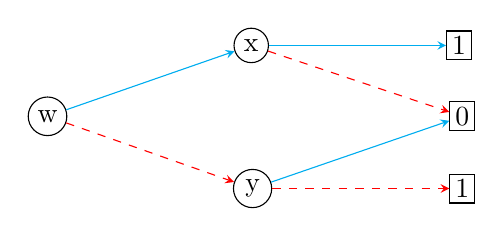
\begin{tikzpicture}[
node distance = 8pt and 64pt,
inner/.style={circle, draw=black, inner sep = 2pt, minimum size = 2pt},
terminal/.style={rectangle, draw=black, inner sep = 2pt, minimum size=2pt},
low/.style ={-stealth,dashed,red},
high/.style = {-stealth, solid,cyan}]

\node[inner] (0c0) {w};
\node[inner] (1c0) [above right = 16pt and 64pt of 0c0] {x};
\node[inner] (1c1) [below right = 16pt and 64pt of 0c0] {y};

\node[terminal] (1) [right = 64pt of 1c0] {1};
\node[terminal] (0) [right = 138pt of 0c0] {0};
\node[terminal] (01) [right = 64pt of 1c1] {1};

\draw[high](0c0)--(1c0);
\draw[low](0c0)--(1c1);

\draw[high](1c0)--(1);
\draw[low](1c0)--(0);

\draw[high](1c1)--(0);
\draw[low](1c1)--(01);
\end{tikzpicture}
\end{center}
The graph shown above is a BDD with non-terminal nodes labeled by variables from $\{w,x,y\}$. It has three terminal nodes, two of them labeled with $1$ and the last labeled with $0$. Lastly, it has three edges of type $1$ and three edges of type $0$. This BDD corresponds to an equivalence class of boolean formulae which contains
$$wx \oplus (w \oplus 1)(y \oplus 1).$$
\end{example}

The ternary \textit{if-then-else} operator $\ite{\cdot}{\cdot}{\cdot} : \{0,1\}^3 \to \{0,1\}$ is defined by 
$$\ite{x}{y}{z} = xy \oplus (1 \oplus x)z$$
where as per usual multiplication has higher precedence than addition. This function returns the value of $y$ if $x=1$ and returns the value of $z$ if $x=0$. One way of viewing binary decision diagrams is as a compressed way of representing boolean formulae built from the if-then-else operator: as a directed acyclic graph rather than as a tree.

\begin{example}
\hfill \\
Formula: $\ite{w}{\ite{x}{\ite{w}{0}{1}}{\ite{y}{1}{0}}}{\ite{y}{0}{1}}$
\begin{center}
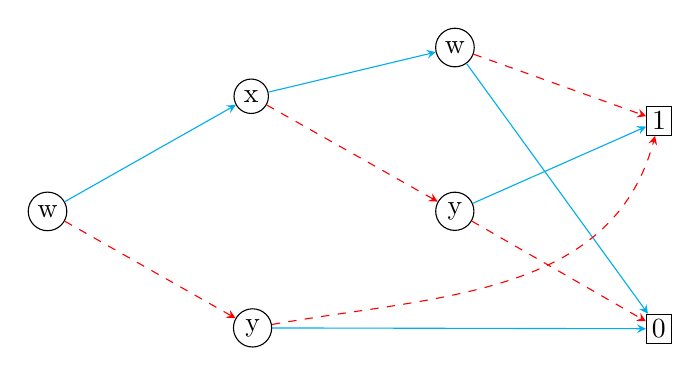
\begin{tikzpicture}[
node distance = 8pt and 64pt,
inner/.style={circle, draw=black, inner sep = 2pt, minimum size = 2pt},
terminal/.style={rectangle, draw=black, inner sep = 2pt, minimum size=2pt},
low/.style ={-stealth,dashed,red},
high/.style = {-stealth, solid,cyan}]

\node[inner] (0c0) {w};
\node[inner] (1c0) [above right = 32pt and 64pt of 0c0] {x};
\node[inner] (1c1) [below right = 32pt and 64pt of 0c0] {y};
\node[inner] (2c0) [above right = of 1c0] {w};
\node[inner] (2c1) [below right = 32pt and 64pt of 1c0] {y};

\node[terminal] (1) [below right = 16pt and 64pt of 2c0] {1};
\node[terminal] (0) [below right = 32pt and 64pt of 2c1] {0};

\draw[high](0c0)--(1c0);
\draw[low](0c0)--(1c1);
\draw[high](1c0)--(2c0);
\draw[low](1c0)--(2c1);

\draw[high](2c0)--(0);
\draw[low](2c0)--(1);
\draw[high](2c1)--(1);
\draw[low](2c1)--(0);

\draw[high](1c1)--(0);
\draw[low](1c1) to[out=10, in=255] (1);
\end{tikzpicture}
\end{center}
\end{example}

The \textit{size} of a BDD is its number of nodes. The BDD shown in Example $2.2$ has size $7$.
\begin{example}
The following BDD has size $4$.
\begin{center}
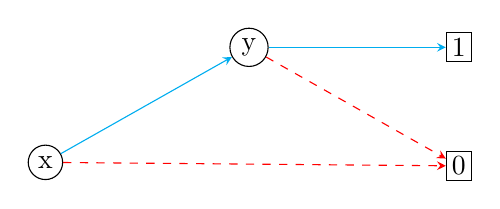
\begin{tikzpicture}[
node distance = 32pt and 64pt,
inner/.style={circle, draw=black, inner sep = 2pt, minimum size = 2pt},
terminal/.style={rectangle, draw=black, inner sep = 2pt, minimum size=2pt},
low/.style ={-stealth,dashed,red},
high/.style = {-stealth, solid,cyan}]

\node[inner] (0c0) {x};
\node[inner] (1c0) [above right = of 0c0] {y};

\node[terminal] (1) [right = of 1c0] {1};
\node[terminal] (0) [below = of 1] {0};

\draw[high](0c0)--(1c0);
\draw[high](1c0)--(1);
\draw[low](0c0)--(0);
\draw[low](1c0)--(0);
\end{tikzpicture}
\end{center}
\end{example}

A BDD is \textit{ordered} and called an \textit{ordered binary decision diagram} (OBDD) if all paths from its root to a terminal node respect a given linear order on its variable labels. For example the BDD shown in example $2.3$ is ordered with respect to the ordering $x<y$ but the BDD in example $2.2$ is not ordered since $w$ appears twice in a path from the root to the $1$-labeled terminal node. 

OBDDs correspond to boolean functions in a manner which is similar to the way that boolean functions correspond to boolean formulae. In an OBDD, every path from the root to a $1$-labeled terminal node corresponds to an assignment for which the corresponding boolean function evaluates to $1$, and every path from the root to a $0$-labeled terminal node corresponds to an assignment for which the corresponding boolean function evaluates to $0$. 

\begin{example}
\hfill \\
\begin{tabular}{l l}
Order: & $w<x<y<z$ \\
Function: & $w \oplus x \oplus y \oplus z $ \\
\end{tabular}
\begin{center}
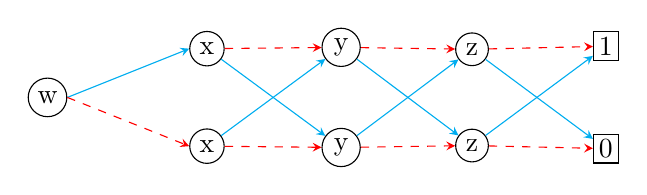
\begin{tikzpicture}[
node distance = 8pt and 32pt,
inner/.style={circle, draw=black, inner sep = 2pt, minimum size = 2pt},
terminal/.style={rectangle, draw=black, inner sep = 2pt, minimum size=2pt},
low/.style ={-stealth,dashed,red},
high/.style = {-stealth, solid,cyan}]

\node[inner] (0c0) {w};
\node[inner] (1c0) [above right = 8 pt and 48pt of 0c0] {x};
\node[inner] (1c1) [below right = 8 pt and 48pt of 0c0] {x};
\node[inner] (2c0) [above right = 8 pt and 96pt of 0c0] {y};
\node[inner] (2c1) [below right = 8 pt and 96pt of 0c0] {y};
\node[inner] (3c0) [above right = 8 pt and 144pt of 0c0] {z};
\node[inner] (3c1) [below right = 8 pt and 144pt of 0c0] {z};
\node[terminal] (1) [above right = 8 pt and 192pt of 0c0] {1};
\node[terminal] (0) [below right = 8 pt and 192pt of 0c0] {0};
\draw[high](0c0.east)--(1c0.west);
\draw[low](0c0.east)--(1c1.west);

\draw[low](1c0)--(2c0);
\draw[high](1c0)--(2c1);
\draw[high](1c1)--(2c0);
\draw[low](1c1)--(2c1);

\draw[low](2c0)--(3c0);
\draw[high](2c0)--(3c1);
\draw[high](2c1)--(3c0);
\draw[low](2c1)--(3c1);

\draw[low](3c0)--(1);
\draw[high](3c0)--(0);
\draw[high](3c1)--(1);
\draw[low](3c1)--(0);
\end{tikzpicture}
\end{center}
The path $w,x,y,z,0$ along only solid arcs corresponds to $w=x=y=z=1$ and reflects $1 \oplus 1 \oplus 1 \oplus 1 = 0$.
\end{example}

An OBDD in the variables $X = \{x_1,\dots,x_m\}$ with order $x_1<\dots<x_m$ defines a boolean function $f$ by the set of paths from its root to a terminal node. If $a_1,\dots,a_m \in \{0,1\}$ with $a_i$ the type of an edge $e_i$ leaving a node $v_i$ with label $x_i$ and $b$ is a terminal node then if $v_1e_1v_2e_2\dots v_me_mb$ is a path in $B$ then the value of $f(a)$, the value of $f$ with each $a_i$ substituted for $x_i$, is the constant labeling $b$. If $v_{i_1}e_{i_1}\dots v_{i_k}e_{i_k}b$ is a path from the root of $B$ to a terminal node $b$ with $x_{i_j}$ the label of $v_{i_j}$ and $a_{i_j}$ the type of $e_{i_j}$ then the partial evaluation of $f$ with $a_{i_j}$ substituted for $x_{i_j}$ evaluates to the value of the constant labeling $b$. Similarly paths from the root of $B$ to some other non-terminal node in $B$ correspond to partial evaluations of $f$ which do not necessarily evaluate to a constant. As the following example shows, partial evaluation is one way in which to build an OBDD for a specified boolean function. 

\begin{example}[Construction]
\hfill \\
\begin{tabular}{l l}
Order: & $w<x<y<z$ \\
Function: & $wx \oplus yz $
\end{tabular}
\begin{center}
\begin{tikzpicture}[
node distance = 48pt and 48pt,
inner/.style={circle, draw=black, inner sep = 2pt, minimum size = 2pt},
terminal/.style={rectangle, draw=black, inner sep = 2pt, minimum size=2pt},
low/.style ={-stealth,dashed,red},
high/.style = {-stealth, solid,cyan}]

\node[inner, label= left: {\small $wx \oplus yz$}] (0c0) {w};
\node[inner, label= above: {\small $x \oplus yz$}] (1c0) [above right = 24pt and 48pt of 0c0] {x};
\node[inner, label= below: {\small $1 \oplus yz$}] (2c0) [right = of 1c0] {y};
\node[inner, label= above: {\small $yz$}] (2c1) [below = of 2c0] {y};
\node[inner, label= above: {\small $1 \oplus z$}] (3c0) [right = of 2c0] {z};
\node[inner, label= below: {\small $z$}] (3c1) [below = of 3c0] {z};
\node[terminal,label= above: {\small $1$}] (1) [right = of 3c0] {1};
\node[terminal,label= below: {\small $0$}] (0) [below = of 1] {0};

\draw[high](0c0)--(1c0);
\draw[high](1c0)--(2c0);
\draw[low](1c0) to[out=310, in=140] (2c1);
\draw[low](0c0) to[out=330, in=180] (2c1);
\draw[high](2c0)--(3c0);
\draw[high](2c1)--(3c1);
\draw[low](2c0) to[out=45, in 135] (1);
\draw[low](2c1) to[out=315, in=225] (0);
\draw[high](3c0)--(0);
\draw[low](3c0)--(1);
\draw[high](3c1)--(1);
\draw[low](3c1)--(0);
\end{tikzpicture}
\end{center}
The boolean formula next to each node is the result of the partial evaluation of the function corresponding to the diagram at every partial evaluation corresponding to a path from the root to that node.
\end{example}

Given an order $\vartriangleleft$ on a set of boolean variables $V$, a \textit{$\vartriangleleft$-OBDD on $V$} is an OBDD in the variables $V$ using the order $\vartriangleleft$. Similarly, a \textit{$\vartriangleleft$-OBDD} is an OBDD using order $\vartriangleleft$ and whose non-terminal nodes are labeled by the elements of some subset of $V$. If $f(v_1,\dots,v_m)$ is a boolean function and $g(v_{i_1},\dots,v_{i_k})$ is a boolean function obtained from $f$ by assigning constant values to a subset of the variables $v_1,\dots,v_m$ then $g$ is called a \textit{subfunction} of $f$.

\begin{example}
If
$$f(v_1,v_2) = v_1 \oplus v_2$$
and
$$g(v_1) = v_1 \oplus 1$$
then $g$ is the subfunction of $f$
$$f(v_1,1).$$
\end{example}

Suppose that $f=f(x_1,\dots,x_m)$ is some boolean function in the variables $x_1,\dots,x_m$. Let $<$ be the ordering on $x_1,\dots,x_m$ given by $x_1<x_2<\dots<x_m$. For $k \in \{1,\dots,m\}$, how many non-terminal nodes are labeled with $x_k$ in the smallest $<$-OBDD for $f$? Due to the correspondence between paths in the $<$-OBDD for $f$ and partial evaluations of $f$, a partial answer to this question is ``at most $|\{f(a_1,\dots,a_{k-1},x_k,\dots,x_m) : a_1,\dots,a_{k-1} \in \{0,1\} \}|$''. For example, consider the boolean function $f(w,x,y,z) = wx \oplus yz$ whose smallest OBDD using ordering $w<x<y<z$ is given in Example 2.5. Since 
$$f(0,x,y,z) = yz \neq x \oplus yz = f(1,x,y,z),$$
there are at most $2$ nodes labeled with $x$ in the OBDD. Similarly, since
$$f(0,0,y,z)=f(1,0,y,z)=f(0,1,y,z)=yz \neq 1 \oplus yz = f(1,1,y,z),$$
there are at most $2$ nodes labeled with $y$ in the OBDD.

\newpage

\section{Results}

\subsection{Quotient and remainder}
Common integer addition and multiplication algorithms, as well as $p$-adic arithmetic algorithms in general, use the concept of carrying. Carrying is based on the idea of iteratively applying the following concept. Given a positive integer $N>1$ and a pair $x,y$ each having an $N$-adic expansion, in order to find the $N$-adic expansion of $x+Ny$ do the following:
\begin{enumerate}
\item Find an $a$ and $b$ and such that $a \in \{0,\dots,N-1\}$, $b$ has an $N$-adic expansion, and $x = a + Nb$.
\item Rewrite $x+Ny$ to $a + N(b+y)$.
\item Find the $N$-adic expansion of $b+y$.
\end{enumerate}
This motivates us to define functions for each positive integer $N>1$, $\re_N$ and $\qu_N$, such that for any $x$ which has an $N$-adic expansion, $\re_N(x) \in \{0,\dots,N-1\}$, $\qu_N(x)$ has an $N$-adic expansion, and $x = \re_N(x) + N\qu_N(x)$.

For every positive integer $N$ let $R_N$ denote the set of all rational numbers $b/a$ with $a,b \in \Z$ such that $\gcd(a,N)=1$ and define the functions $\re_N$ and $\qu_N$ by the following:
\begin{itemize}
\item  $\re_N : R_N \rightarrow \{0,...,N-1\}$ and for all $w,x,y \in \Z$ such that $\gcd(x,N)=1$ and $w \in \{0,\dots,N-1\}$,
$$\re_N(y/x) = w \ \iff \ y \equiv wx \pmod{N}.$$
\item $\qu_N : R_N \to R_N$ and for all $y \in R_N$
$$\qu_N(y) = \frac{y-\re_N(y)}{N}.$$
\end{itemize}
For each $x$, $\qu_N(x)$ will be referred to as \textit{the quotient of $x$ with respect to $N$} or simply \textit{the quotient of $x$} if $N$ is known from the context. Likewise, $\re_N(x)$ will be referred to as \textit{the remainder of $x$ with respect to $N$} or more simply \textit{the remainder of $x$} if $N$ is understood. 

The following proposition shows that quotient and remainder functions have nice properties which allow us to efficiently apply them to the result of an arithmetic operation provided we know their value on the inputs to the arithmetic operation as well as a small bounded set of input values.

\begin{proposition}
For all $N, \alpha,\beta \in \N$ and for all $x,y \in R_N$, $\re_N$ and $\qu_N$ satisfy:
\begin{enumerate}
\item $\re_N(x \pm y) = \re_N(x \pm \re_N(y))$
\item $\re_N(xy) = \re_N(\re_N(x)y)$
\item $\re_{N^{\alpha}} ( \re_{N^{\beta}}(x) ) = \re_{N^{\textrm{min}(\alpha,\beta)}}(x)$
\item $\qu_N(x \pm y) = \qu_N(x \pm \re_N(y)) \pm \qu_N(y)$
\item $\qu_N(xy) = \qu_N(x)y+\qu_N(\re_N(x)y)$
\item $\qu_{N^{\alpha}} ( \qu_{N^{\beta}}(x) ) = \qu_{N^{\alpha+\beta}}(x)$
\item $x = N^{\beta}\qu_{N^{\beta}}(x)+\sum_{k=0}^{\beta - 1}\re_N(\qu_{N^k}(x))N^k$
\item $(x,y \in \Z \ \land \ x \leq y) \implies (\qu_N(x) \leq \qu_N(y))$
\item $\re_N(-1-x) = N-1-\re_N(x)$
\end{itemize}
If $N$ is prime then the preceding holds for all $x,y \in \Z_N$ and in addition if $\alpha \leq \beta$ then
$$\qu_{N^{\alpha}}(\re_{N^{\beta}}(x)) = \re_{N^{\beta-\alpha}}(\qu_{N^{\alpha}}(x)).$$
\end{proposition}

\begin{proof}
Note that $R_1 = \Q$ and for all $w \in \Q$ $\re_1(w) = 0$  and $\qu_1(w) = w$. Thus if $N=1$ then $1$ through $8$ hold.

Suppose that $N>1$ is a positive integer, $x,y \in R_N$, and $\alpha,\beta \in \N$. Statements $1$ and $2$ follow from the fact that congruence mod $N$ respects addition, subtraction, and multiplication. If $\alpha \leq \beta$ then it follows from $1$ and $2$ that
\begin{align*}
\re_{N^{\alpha}}(\re_{N^{\beta}}(x)) &= \re_{N^{\alpha}}(\re_{N^{\beta}}(x) + N^{\beta}\qu_{N^{\beta}}(x)) \\
&= \re_{N^{\alpha}}(x) \\
&= \re_{N^{\textrm{min}(\alpha,\beta)}}(x).
\end{align*}
If $\alpha > \beta$ then since $\{0,\dots,N^{\beta}-1\} \subset \{0,\dots,N^{\alpha}-1\}$,
\begin{align*}
\re_{N^{\alpha}}(\re_{N^{\beta}}(x)) &= \re_{N^{\beta}}(x) \\
&= \re_{N^{\textrm{min}(\alpha,\beta)}}(x).
\end{align*}
Therefore $3$ holds. To see that $4$ holds, observe that
\begin{align*}
\qu_N(x+y) &= \frac{x+y-\re_N(x+y)}{N} \\
&= \frac{x+y-\re_N(y)+\re_N(y)-\re_N(x+\re_N(y))}{N} \\
&= \frac{x+\re_N(y)-\re_N(x+\re_N(y))}{N} + \frac{y-\re_N(y)}{N} \\
&= \qu_N(x+\re_N(y)) + \qu_N(y)
\end{align*}
and
\begin{align*}
\qu_N(x-y) &= \frac{x-y-\re_N(x-y)}{N} \\
&= \frac{x-(y-\re_N(y)+\re_N(y))-\re_N(x-\re_N(y))}{N} \\
&= \frac{x-\re_N(y)-\re_N(x-\re_N(y))}{N}-\frac{y-\re_N(y)}{N} \\
&= \qu_N(x-\re_N(y))-\qu_N(y).
\end{align*}
The proof of $5$ is another derivation similar to that for $4$:
\begin{align*}
\qu_N(xy) &= \frac{xy - \re_N(xy)}{N} \\
&= \frac{N\qu_N(x)y + \re_N(x)y - \re_N(\re_N(x)y)}{N} \\
&= \qu_N(x)y + \frac{\re_N(x)y - \re_N(\re_N(x)y)}{N} \\
&= \qu_N(x)y+\qu_N(\re_N(x)y).
\end{align*}
For the proof of $6$ first observe that
\begin{align*}
x &= \re_{N^{\beta}}(x) + N^{\beta} \qu_{N^{\beta}}(x) \\
&= \re_{N^{\beta}}(x) + N^{\beta} \re_{N^{\alpha}}(\qu_{N^{\beta}}(x)) + N^{\beta + \alpha}\qu_{N^{\alpha}}(\qu_{N^{\beta}}(x)).
\end{align*}
Therefore since
$$ \re_{N^{\beta}}(x) + N^{\beta} \re_{N^{\alpha}}(\qu_{N^{\beta}}(x)) \leq N^{\beta}-1 +  N^{\beta}(N^{\alpha}-1) = N^{\beta + \alpha} - 1$$
it follows that
$$ \re_{N^{\beta+\alpha}}(x) =  \re_{N^{\beta}}(x) + N^{\beta} \re_{N^{\alpha}}(\qu_{N^{\beta}}(x)). $$
And so
$$\qu_{N^{\alpha}} ( \qu_{N^{\beta}}(x) ) = \qu_{N^{\alpha+\beta}}(x).$$
We use statement $6$ to prove $7$ by induction. For the base case observe
$$x = \re_{N}(x) + N\qu_{N}(x).$$
For the inductive step, suppose that $m$ is a positive integer and
$$x = N^{m}\qu_{N^{m}}(x)+\sum_{k=0}^{m - 1}\re_N(\qu_{N^k}(x))N^k.$$
It follows that
\begin{align*}
x &= N^{m}\qu_{N^{m}}(x)+\sum_{k=0}^{m - 1}\re_N(\qu_{N^k}(x))N^k \\
 &= N^{m}(N\qu_{N}(\qu_{N^{m}}(x)) + \re_N(\qu_{N^{m}}(x)))+\sum_{k=0}^{m - 1}\re_N(\qu_{N^k}(x))N^k \\
&= N^{m+1}\qu_{N^{m+1}}(x)) + N^{m}\re_N(\qu_{N^{m}}(x)))+\sum_{k=0}^{m - 1}\re_N(\qu_{N^k}(x))N^k \\
&= N^{m+1}\qu_{N^{m+1}}(x)) + \sum_{k=0}^{(m+1) - 1}\re_N(\qu_{N^k}(x))N^k.
\end{align*}

For statement $8$, observe that if $w \in \Z$ then
$$\qu_N(w) = \left \lfloor \frac{w}{N} \right \rfloor.$$
Since $w \mapsto \left \lfloor \frac{w}{N} \right \rfloor$ is an increasing function, $8$ follows immediately.

Finally, for statement $9$ observe that for $x \in R_N$ since $\re_N(x) \in \{0,\dots,N-1\}$, $N-1-\re_N(x) \in \{0,\dots,N-1\}$, and so
$$N-1-\re_N(x) = \re_N(N-1-\re_N(x)) = \re_N(-1-x).$$

Suppose that $N$ is prime and $\alpha \leq \beta$. It is evident from the preceding that for $x \in \Z_N$ 
$$x = \sum_{k \geq 0}\re_N(\qu_{N^{k}}(x))N^k,$$
$$\re_{N^{\alpha}}(x) = \sum_{k=0}^{\alpha-1}\re_N(\qu_{N^{k}}(x))N^k,$$
and
$$\qu_{N^{\alpha}}(x) = \sum_{k \geq \alpha}\re_N(\qu_{N^{k}}(x))N^{k - \alpha}.$$
A direct derivation gives, for $\alpha \leq \beta$,
\begin{align*}
\qu_{N^{\alpha}}(\re_{N^{\beta}}(x)) &= \qu_{N^{\alpha}} \left (  \sum_{k=0}^{\beta-1}\re_N(\qu_{N^{k}}(x))N^k \right ) \\
&= \sum_{k=\alpha}^{\beta-1}\re_N(\qu_{N^{k}}(x))N^{k-\alpha} \\
&= \sum_{k=0}^{\beta-\alpha-1}\re_N(\qu_{N^{k+\alpha}}(x))N^{k} \\
&= \sum_{k=0}^{\beta-\alpha-1}\re_N(\qu_{N^{k}}(\qu_{N^{\alpha}}(x)))N^{k} \\
&= \re_{N^{\beta-\alpha}}(\qu_{N^{\alpha}}(x)).
\end{align*}
\end{proof}
Properties 1, 2, 4, 5, 6, and the last unnumbered property following 9 are particularly important in proving results found in sections 3.4 and 3.5.

The following proposition establishes another property of the quotient and remainder functions which is needed to prove a result in section 3.4.
\begin{proposition}
For all $N \in \N$ and for all $x,y \in R_N$, $\re_N$ and $\qu_N$ satisfy
$$\qu_N(x) =\qu_N(x-y) + \qu_N(y+\re_N(-1-x)).$$
Furthermore if $N$ is prime then the preceding equation holds for all $x,y \in \Z_N$.
\end{proposition}
\begin{proof}
Let $N \in \N$ and $x,y \in R_N$. If $N=1$ then then
$$\qu_N(x) = x = x-y+y+0 = \qu_N(x-y) + \qu_N(y+0) = \qu_N(x-y) + \qu_N(y+\re_N(-1-x)).$$
Suppose that $N>1$. It follows from Proposition $1$ and the fact that for all $w \in R_N$ $\qu_N(\re_N(w))=0$ that
\begin{align*}
\qu_N(x-y)+\qu_N(y+\re_N(-1-x)) &= \qu_N(x-y + N\qu_N(y+\re_N(-1-x))) \\
&= \qu_N(x-y+y+\re_N(-1-x)-\re_N(y-1-x)) \\
&= \qu_N(x+\re_N(-1-x) - \re_N(-1-(x-y))) \\
&= \qu_N(x + N-1-\re_N(x) - (N-1-\re_N(x-y))) \\
&= \qu_N(x-\re_N(x) + \re_N(x-y)) \\
&= \qu_N(N\qu_N(x)+\re_N(x-y)) \\
&= \qu_N(x) + \qu_N(\re_N(x-y)) \\
&= \qu_N(x).
\end{align*}
Since the preceding derivation only relied on the fact that $N>1$ and $x,y$ were in the domain of $\qu_N$ and $\re_N$ it holds when $N$ is prime and $R_N$ is replaced by $\Z_N$. 
\end{proof}

\subsection{Digit Recurrences}
Let $p \in \N$ be prime. We will refer to a recurrence relation for the $n$th $p$-adic digit of the result of an arithmetic operation in terms of the $p$-adic digits of its inputs as a \textit{$p$-adic digit recurrence relation}.

In this section we present a collection of $p$-adic digit recurrence relations, one for each arithmetic operation. It is shown how these recurrences can be converted from equations interpreted in $\Q$ or $\Z_p$ to congruences modulo $p$. This generalizes previous work on the subject for the specific case that $p=2$ \cite{Lomonaco}. 

First note that it is straightforward to obtain polynomials interpolating $\qu_p$ and $\re_p$ on 
$$\{a \star b \ \mid \ a,b \in \{0,\dots,p-1\} \}$$
where $\star \in \{{}+{},{}-{},{}\times{},{}/{}\}.$ In addition, for $t \in \Z_p$ and $n \in \N_0$, the $n$th $p$-adic digit of $t$ is given by $\re_p ( \qu_{p^n}(t) )$. Therefore given $t \in \Z_p$ and a recurrence for $\qu_{p^n}(t)$, a recurrence for the $n$th $p$-adic digit of $t$ is obtained immediately from $\re_p ( \qu_{p^n}(t) )$.

Let $x,y \in \Z_p$, and let $(x_n)_{n\geq0}$ and $(y_n)_{n\geq0}$ be the $p$-adic digit vectors associated to, respectively, $x$ and $y$. For each $m \in \Z$ such that $m<0$ define $x_m=y_m=0$.

In order to streamline the presentation of some of the recurrences we will extend $\qu_{p^m}$ and $\re_{p^m}$ to allow for negative integers $m$. For each $m \in \Z$ if $m<0$ then for all $t \in \Z_p$ let 
$$\qu_{p^m}(t) = p^{-m}t \ \land \ \re_{p^{m}}(t) = 0$$
\begin{itemize}
\item [Addition:] 
\begin{align*}
\qu_{p^n}(x+y) &= \qu_{p^n}(x)+\qu_{p^n}(y) + z_n \\
z_n &= \qu_p(x_{n-1}+y_{n-1}) + \qu_p(\re_p(x_{n-1}+y_{n-1})+1)z_{n-1} \\
n \leq 0 &\implies z_n = 0
\end{align}

\item [Subtraction:] 
\begin{align*}
\qu_{p^n}(x-y) &= \qu_{p^n}(x)-\qu_{p^n}(y) + z_n \\
z_n &= \qu_p(x_{n-1}-y_{n-1}) - \qu_p(\re_p(x_{n-1}-y_{n-1})-1)z_{n-1} \\
n \leq 0 &\implies z_n = 0
\end{align}

\item [Multiplication:]
\begin{align*}
\qu_{p^n}(xy) &= \qu_{p^n}(x)y + a_{n,n-1} \\
a_{m,n} &= a_{m,n-1}+b_{m-n,n}+c_{m,n} \\
b_{m,n} &= \qu_{p^m}(y)x_n + \qu_p(x_n y_{m-1}) + d_{m-1,n} \\
d_{m,n} &= \qu_{p}(\re_p(x_n y_{m-1}) + \qu_p(x_n y_{m-1})) + \qu_{p}(\re_p(x_n y_{m-1} + \qu_p(x_n y_{m-1})) + 1)d_{m-1,n} \\
c_{m,n} &= \qu_p ( \re_p(a_{m-1,n-1}) + \re_p(b_{m-1-n,n}) ) + \qu_p (\re_p(a_{m-1,n-1} + b_{m-1-n,n}) + 1)c_{m-1,n} \\
n < 0 &\implies a_{m,n} = 0 \\
n < 0 &\implies b_{m,n} = 0 \\
n \leq 0 &\implies c_{m,n} = 0 \\
n < 0 &\implies d_{m,n} = 0 \\
b_{0,n} &= x_n y \\
c_{0,n} &= 0 \\
d_{0,n} &= 0 \\
\end{align}
Note that for any $u,v \in \{0,\dots,p-1\}$ $\qu_p(uv) \in \{0,\dots,p-2\}$.

\item [Division:]
\begin{align*}
\qu_{p^n} \left ( \frac{y}{x} \right ) &= \frac{z_{0,n}}{x} \\
z_{m,n} &= z_{m+1,n-1} - a_{m+1,n-1} + b_{m,n-1} \\
a_{m,n} &= \qu_{p^m}(x)\re_{p}\left ( \frac{z_{0,n}}{x_0} \right ) + \qu_p \left ( x_{m-1} \re_{p}\left ( \frac{z_{0,n}}{x_0} \right ) \right ) + c_{m-1,n} \\
c_{m,n} &= \qu_p \left ( \re_p \left ( \frac{ x_m z_{0,n}}{x_0} \right ) + \qu_p \left ( x_{m-1}\re_{p}\left ( \frac{z_{0,n}}{x_0} \right ) \right ) \right ) \\
        & \ \ + \qu_p \left ( \re_p \left ( \frac{ x_m z_{0,n}}{x_0} + \qu_p \left ( x_{m-1} \re_{p} \left ( \frac{z_{0,n}}{x_0} \right ) \right ) \right ) + 1 \right ) c_{m-1,n} \\
b_{m,n} &= \qu_p(\re_p(z_{m,n}) - \re_p(a_{m,n})) - \qu_p(\re_p(z_{m,n} - a_{m,n})-1)b_{m-1,n} \\
m \leq 0 &\implies b_{m,n} = 0 \\
m \leq 0 &\implies c_{m,n} = 0 \\
z_{m,0} &= \qu_{p^m}(y)
\end{align}
where it is assumed that $\gcd(x_0,p)=1$.

\end{itemize}

We note that the recurrences for addition and subtraction are analogous to equations describing a binary carry-save adder. The variable $z_n$ in the addition and subtraction recurrences represents the carry to $p^n$, i.e. 
$$z_n = \qu_{p^n}(\re_{p^n}(x) \pm \re_{p^n}(y)).$$

The multiplication recurrence corresponds to a method of multiplication commonly taught in primary school which is sometimes referred to as \textit{long multiplication}. The variable $a_{m,n}$ represents the quantity carried to $p^m$ from $A_n = \sum_{k=0}^{n}[x_kp^k]y$, $a_{m,n} = \qu_{p^m}(\re_{p^{n+1}}(x)y)$. In order to calculate $a_{m,n}$ we rewrite $A_n$ as the sum of two quantities, $A_n = A_{n-1} + x_np^ny$, then apply the addition recurrence. The variable $c_{m,n}$ tracks the carried quantities to $p^m$ in the summation $A_{n-1} + x_np^ny$ while $b_{m,n}$ and $d_{m,n}$ are used in determining the $p$-adic expansion of $x_np^ny$, as it is needed to determine $c_{m,n}$.

The recurrence for division is based on the following: assuming that $x$ is a unit in $\Z_p$,
$$y/x = \re_{p^n}(y/x) +p^nz_n/x \iff z_n = x \qu_{p^n}(y/x)$$
So let $z_n = x \qu_{p^n}(y/x)$ then
\begin{align*}
z_n &= x \qu_{p^n}(y/x) \\
 &= x \qu_{p}(\qu_{p^{n-1}}(y/x)) \\
 &= x\qu_p(z_{n-1}/x).
\end{align}
In the appendix it is shown that 
$$x\qu_p(z_{n-1}/x) = \qu_p(z_{n-1}) - \qu_p(\re_p(z_{n-1}/x)x);$$
so then $z_n = \qu_p(z_{n-1}) - \qu_p(\re_p(z_{n-1}/x)x)$. From this point we let $z_{m,n} = \qu_{p^m}(z_n)$ and then find a recurrence for $z_{m,n}$. Like multiplication, this involves invoking the recurrences for addition and subtraction, as well as for quantities of the form $\qu_{p^m}(au)$ where $a \in \{0,\dots,p-1\}$ and $u \in \Z_p$.

Derivations for the presented recurrence relations are rather straightforward, following from properties of the $\re_p$ and $\qu_p$ functions given in Proposition $1$. For completeness, an outline of their derivations can be found in appendix A.

Lucas' Theorem allows us to convert these recurrences to congruences modulo $p$ due to its implication that for each $x \in \Z_p$ and $n \in \N_0$,
$$\re_p(\qu_{p^n}(x)) = \re_p \left ( \binom{x}{p^n} \right )$$
or in other words
$$\qu_{p^n}(x) \equiv \binom{x}{p^n} \pmod{p}.$$
Note that for $m \in \N_0$ if $m \leq p-1$ then
$$\binom{x}{m} \equiv_p \frac{\prod_{k=0}^{m-1}[x-k]}{m!};$$
that is, we need not worry about division by zero mod $p$. Furthermore the Chu-Vandermonde identity states that for $c \in \N_0$
$$\binom{a+b}{c} = \sum_{n \geq 0} \binom{a}{n}\binom{b}{c-n}$$
While the Newton series for $\binom{ab}{c}$ implies that for all $a,b,c \in \N_0$,
$$\binom{ab}{c} = \sum_{i,j \in \N_0}\binom{a}{i}\binom{b}{j}\sum_{k,l \in \N_0}(-1)^{i+j-k-l}\binom{i}{k}\binom{j}{l}\binom{kl}{c},$$
noting that for all $n$ and for all $m \in \Z$, if $m<0$ then $\binom{n}{m}=0$. These facts taken together have useful implications. For example,
\begin{align*}
\qu_{p}(\re_p(x)+\re_p(y)) &\equiv_p \binom{\re_p(x)+\re_p(y)}{p} \\
 &= \sum_{k=0}^{p}\binom{\re_p(x)}{k}\binom{\re_p(y)}{p-k} \\
 &= \sum_{k=1}^{p-1}\binom{\re_p(x)}{k}\binom{\re_p(y)}{p-k} \\
 &\equiv_p \sum_{k=1}^{p-1}\binom{x}{k}\binom{y}{p-k}
\end{align*}
and
\begin{align*}
\qu_{p}(\re_p(x)\re_p(y)) &\equiv_p \binom{\re_p(x)\re_p(y)}{p} \\
 &= \sum_{i=1}^{p-1}\sum_{j=1}^{p-1}\binom{\re_p(x)}{i}\binom{\re_p(y)}{j}\sum_{k=1}^{p-1}\sum_{l=1}^{p-1}(-1)^{i+j-k-l}\binom{i}{k}\binom{j}{l}\binom{kl}{p} \\
&\equiv_p \sum_{i=1}^{p-1}\sum_{j=1}^{p-1}\binom{x}{i}\binom{y}{j}\sum_{k=1}^{p-1}\sum_{l=1}^{p-1}(-1)^{i+j-k-l}\binom{i}{k}\binom{j}{l}\binom{kl}{p}.
\end{align*}

\begin{example}
Suppose $p=2$, then the recurrences for addition and subtraction can be expressed as the following congruences.
\begin{itemize}
\item[Addition:]
\begin{align*}
\binom{x+y}{2^n} &\equiv_2 x_n + y_n + z_n \\
z_n &\equiv_2 x_{n-1}y_{n-1} + (x_{n-1}+y_{n-1})z_{n-1}.
\end{align}

\item[Subtraction:]
\begin{align*}
\binom{x-y}{2^n} &\equiv_2 x_n - y_n + z_n \\
z_n &\equiv_2 (1+x_{n-1})y_{n-1} + (1+x_{n-1}+y_{n-1})z_{n-1} .
\end{align}

Furthermore the recurrence relations for multiplication and division simplify a great deal since the range of $\re_2$ is $\{0,1\}$. Notably for all $x,y \in \Z_2$ and $n \in \N_0$
\begin{align*}
\qu_{2^n}(\re_2(x)y) &= \re_2(x)\qu_{2^n}(y), \\
\qu_2(\re_2(x) + \re_2(y)) &= \re_2(x)\re_2(y), \\
\qu_2(\re_2(x) - \re_2(y)) &= -(1-\re_2(x))\re_2(y).
\end{align}
This allows us to express the recurrences for multiplication and division as the following congruences:
\begin{itemize}
\item[Multiplication:]
\begin{align*}
\binom{xy}{2^n} &\equiv_2 x_ny_0 + a_{n,n-1} \\
a_{m,n} &\equiv_2 a_{m,n-1} + x_ny_{m-n} + c_{m,n} \\
c_{m,n} &\equiv_2 a_{m-1,n-1}x_n y_{m-1-n} + (a_{m-1,n-1}+x_n y_{m-1-n})c_{m-1,n} \\
n < 0 &\implies a_{m,n} \equiv_2 0 \\
n < 0 &\implies c_{m,n} \equiv_2 0 ;
\end{align}

\item[Division:]
\begin{align*}
\binom{y/x}{2^n} &\equiv_2 \frac{z_{0,n}}{x} \\
z_{m,n} &\equiv_2 z_{m+1,n-1} + x_{m+1}z_{0,n-1} + b_{m,n-1} \\
b_{m,n} &\equiv_2 x_mz_{0,n}(1+z_{m,n}) + (x_mz_{0,n} + 1 + z_{m,n})b_{m-1,n} \\
z_{m,0} &\equiv_2 y_m \\
b_{0,n} &\equiv_2 0.
\end{align}
\end{itemize}

\end{example}

\subsection{Digit Formulae}
Before diving into this section it is necessary to introduce some notation. The symbol $\emptyset$ is used to denote both the empty set as well as the empty function whose codomain will be apparent from the context. For example $\mathbbm{N}^{0}$ represents the singleton containing the empty function with codomain $\mathbbm{N}$. Let $T$ be a set with finite cardinality. A summation over an empty indexing set is taken to be $0$ and a product taken over an empty indexing set is taken to be $1$. Let $a,b : T \to \mathbbm{N}_0$. When  $a$ and $b$ are used to describe the indexing set of a summation or product we will observe the following notational conventions:
$$a_i = a(i) \ \textrm{whenever} \ i \in T,$$
$$a \pm b = (a_i \pm b_i)_{i \in T},$$
and
$$|a| = \sum_{i \in T} a_i \ \textrm{where} \ |\emptyset| = 0.$$

We now show how binomial coefficients can be used to give an explicit description of the $n$th $p$-adic digit of an element $z \in \Z_p$ whenever it is presented as a series of the form $\sum_{k \geq 0}z_kp^k$ where each $z_k \in \Z_p$. Descriptions of solutions to the $p$-adic digit recurrence relations follow from this as given $x,y \in \Z_p$ with associated $p$-adic digit vectors $(x_n)_{n \geq 0}$ and $(y_n)_{n \geq 0}$, we have
\begin{align*}
x \pm y &= \sum_{n \geq 0}(x_n \pm y_n)p^n ,\\
xy &= \sum_{n \geq 0}\sum_{m=0}^{n}x_my_{n-m}p^n.
\end{align*} 
If $x_0 \neq 0$ then we have
$$y/x = \sum_{n \geq 0} \left [ \sum_{m=0}^{n} \left ( y_{n-m} \sum_{l \in \textrm{Part}_m}\left [ (-1)^{|l|}\binom{|l|}{l}x_0^{-1-|l|}\prod_{k=1}^{m}x_k^{l_k} \right ] \right ) p^n \right ],$$
where $\textrm{Part}_m = \{l \in \N_0^m \mid \sum_{j=1}^{m}jl_j = m \}$.

\begin{theorem}
If $z \in \Z_p$, for every $k \in \N_0$ $z_k \in \Z_p$, and
$$z = \sum_{k \geq 0} z_kp^k$$
then for all $y, N \in \N_0$ such that $y \leq p^{N+1}-1$,
\begin{align*}
\binom{z}{y} &\equiv_{p} \sum_{\substack{i \in \N_0^{\{0,\dots,N\}} \\ \sum_{j=0}^{N}i_jp^j = y}} \prod_{j=0}^{N}\binom{z_j}{i_j} \\
\end{align}
\end{theorem}

\begin{proof}
We use Lucas' Theorem together with the Chu-Vandermonde identity. Note that for $y,m,n \in \N_0$, if $n \geq m$ then
$$\binom{z}{p^m} \equiv_p \binom{\sum_{k=0}^{n}z_kp^k}{p^m},\textrm{ and}\\$$
$$\binom{p^nz}{p^my} \equiv_p \binom{p^{n-m}z}{y}.$$
The Chu-Vandermonde identity implies
\begin{align*}
\binom{a_1+a_2+\dots + a_m}{c} &= \sum_{n \in \N_0^{m-1}}\binom{a_1}{n_1}\binom{a_2}{n_2} \dots \binom{a_{m-1}}{n_{m-1}}\binom{a_m}{c-n_1-n_2-\dots-n_{m-1}} \\
 &= \sum_{\substack{n \in \N_0^m \\ |n| = c}} \prod_{j=1}^{m}\binom{a_j}{n_j},
\end{align*}
which further implies that
\begin{align*}
\binom{z}{y} &= \sum_{\substack{i \in \N_0^{\{0,\dots,N\}} \\ |i| = y}} \prod_{j=0}^{N}\binom{z_jp^j}{i_j} \\
&\equiv_{p} \sum_{\substack{i \in \N_0^{\{0,\dots,N\}} \\ \sum_{j=0}^{N}i_jp^j = y}} \prod_{j=0}^{N}\binom{z_j}{i_j}.
\end{align*}
\end{proof}

It follows that for each arithmetic operation $\star$, an associated sequence of polynomials is given by
$$((x_n)_{n \geq 0},(y_n)_{n \geq 0}) \mapsto \left ( \sum_{\substack{i \in \N_0^{\{0,\dots,n\}} \\ \sum_{j=0}^{n}i_jp^j = p^n}} \prod_{j=0}^{n}\binom{z_j}{i_j}} \right )_{n \geq 0}$$
where for each $n \in \N_0$
$$z_n = \begin{cases} x_n \pm y_n &\impliedby \star = \pm \\
\sum_{m=0}^{n}x_my_{n-m} &\impliedby \star = \times \\
\sum_{m=0}^{n} x_{n-m} \sum_{l \in \textrm{Part}_m}(-1)^{|l|}\binom{|l|}{l}y_0^{-1-|l|}\prod_{k=1}^{m}y_k^{l_k} &\impliedby \star = /.
\end{cases}$$
It should be noted that there are other choices of polynomial sequences we can use. Since one will no doubt be working with congruences modulo $p$ rather than integer equalities, the exact choice of representative is not all that important. Regardless, with this we have achieved the first goal of this research project, which was to provide a method of obtaining an associated sequence of polynomials for each arithmetic operation on $\Z_p$, in a manner distinct from simulating arithmetic algorithms or digital adder and multiplier circuits.

\begin{example}
Take $p=2$ and $x,y \in \Z_2$ with $2$-adic digit vectors $(x_n)_{n \geq 0}$, and $(y_n)_{n \geq 0}$. Note that for any $(a_1,\dots,a_n) \subseteq \{0,1\}$ and $m \in \N_0$,
$$\binom{\sum_{k=1}^{n}a_k}{m} = \ele_m(a_1,\dots,a_n) = \sum_{0 < k_1 < \dots < k_m < n+1}a_{k_1}\dots a_{k_m}.$$
We calculate polynomials congruent to the $0$th through $3$rd $p$-adic digits of $xy$.
\begin{align*}
\binom{xy}{1} &\equiv_2 \binom{x_0y_0}{1} \\
 &\equiv_2 x_0y_0 \\
\binom{xy}{2} &\equiv_2 \binom{x_0y_0 + 2(x_0y_1 + x_1y_0)}{2} \\
 &\equiv_2 \sum_{k_0+2k_1 = 2}\binom{x_0y_0}{k_0}\binom{x_0y_1 + x_1y_0}{k_1} \\
 &\equiv_2 \binom{x_0y_1 + x_1y_0}{1} \\
 &\equiv_2 x_0y_1 + x_1y_0 \\
\binom{xy}{2^2} &\equiv_2 \binom{x_0y_0 + 2(x_0y_1 + x_1y_0) + 2^2(x_0y_2 + x_1y_1 + x_2y_0)}{2^2} \\
 &\equiv_2 \sum_{k_0+2k_1+2^2k_2 = 2^2}\binom{x_0y_0}{k_0}\binom{x_0y_1 + x_1y_0}{k_1}\binom{x_0y_2 + x_1y_1 + x_2y_0}{k_2} \\
 &\equiv_2 \binom{x_0y_1 + x_1y_0}{2} + \binom{x_0y_2 + x_1y_1 + x_2y_0}{1} \\
 &\equiv_2 x_0y_1x_1y_0 + x_0y_2 + x_1y_1 + x_2y_0 
\end{align*}
\begin{align*}
\binom{xy}{2^3} &\equiv_2 \binom{x_0y_0 + 2(x_0y_1 + x_1y_0) + 2^2(x_0y_2 + x_1y_1 + x_2y_0) + 2^3(x_0y_3+x_1y_2+x_2y_1+x_3y_0)}{2^3} \\
 &\equiv_2 \sum_{k_0+2k_1+2^2k_2+2^3k_3 = 2^3}\binom{x_0y_0}{k_0}\binom{x_0y_1 + x_1y_0}{k_1}\binom{x_0y_2 + x_1y_1 + x_2y_0}{k_2}\binom{x_0y_3+x_1y_2+x_2y_1+x_3y_0}{k_3} \\
 &\equiv_2 \binom{x_0y_1 + x_1y_0}{2}\binom{x_0y_2 + x_1y_1 + x_2y_0}{1} + \binom{x_0y_2 + x_1y_1 + x_2y_0}{2}+\binom{x_0y_3+x_1y_2+x_2y_1+x_3y_0}{1} \\
 &\equiv_2 x_0y_1x_1y_0(x_0y_2 + x_1y_1 + x_2y_0) + x_0y_2x_1y_1 + x_0y_2x_2y_0 + x_1y_1x_2y_0 + x_0y_3+x_1y_2+x_2y_1+x_3y_0 \\
 &\equiv_2 x_0y_1x_1y_0(y_2 + 1+ x_2) + x_0y_2x_1y_1 + x_0y_2x_2y_0 + x_1y_1x_2y_0 + x_0y_3+x_1y_2+x_2y_1+x_3y_0.
\end{align*}
\end{example}

With the preceding example in mind, it is clear how the elementary symmetric polynomials are related to sequences of polynomials associated with arithmetic operations on $\Z_p$. If $m,n \in \N_0$ then $\binom{n}{m} = \ele_m[(1)_{k=1}^{n}]$. The $n$th $p$-adic digit of $x \in \Z_p$ is congruent to $\binom{\re_{p^{n+1}}(x)}{p^n}$ modulo $p$ and $\re_{p^{n+1}}(x) \in \N_0$. Therefore the $n$th $p$-adic digit of $x$ is congruent to $\ele_m[(1)_{k=1}^{N_x}]$ modulo $p$ where $N_x = \re_{p^{n+1}}(x)$. With this relationship established we have now obtained an answer to the second problem statement of this thesis.

\subsection{FACT as a System of Congruences}
In this section we give a flexible method of representing FACT as a system of polynomial function congruences. Within this section $p$ represents an arbitrary prime.

\begin{lemma}
Suppose that $z \in \N_0$, for each $n \in \N_0$ $b_n,z_n \in \N_0$ and $z_n \leq b_n$, and 
$$z = \sum_{n \geq 0}p^nz_n .$$
For each $m,n \in \N_0 \cup \{\infty\}$ such that $m \leq n$ let 
$$Z_{m,n} = \sum_{k=m}^{n}p^{k-m}z_k$$
and let 
$$Z_{n+1,n} = 0 .$$
For each $n \in \N_0$ let $u_n$ denote the largest $m \in \Z$ such that $-1 \leq m \leq n$ and
$$\sum_{k=0}^{m}p^kb_k < p^n$$
where
$$\sum_{k=0}^{-1}p^kb_k=0 .$$

For each $n \in \N_0$ if $m \in \Z$ is such that $-1 \leq m \leq u_n$ then
$$\binom{z}{p^n} \equiv_p \binom{Z_{m+1,n}+\qu_{p^{m+1}}(\re_{p^{n}}(-1-z))}{p^{n-1-m}}.$$
\end{lemma}

\begin{proof} Suppose that $n \in \N_0$ and $m \in \Z$ is such that $-1 \leq u_n$. First notice that it follows from the definition of $u_n$ that 
$$\qu_{p^{n}}(Z_{0,m}) = 0.$$
It follows from propositions $1$ and $2$ of section $3.1$ that
\begin{align*}
\qu_{p^n}(z) &= \qu_{p^n}(z-p^{m+1}Z_{m+1,\infty}) + \qu_{p^n}(p^{m+1}Z_{m+1,\infty} + \re_{p^n}(-1-z)) \\
&= \qu_{p^n}(Z_{0,m}) + \qu_{p^n}(p^{m+1}Z_{m+1,\infty} + \re_{p^n}(-1-z)) \\
&= \qu_{p^n}(p^{m+1}Z_{m+1,\infty} + \re_{p^n}(-1-z)) \\
&= \qu_{p^{n-1-m}}(\qu_{p^{1+m}}(p^{m+1}Z_{m+1,\infty} + \re_{p^n}(-1-z))) \\
&= \qu_{p^{n-1-m}}(Z_{m+1,\infty} + \qu_{p^{1+m}}(\re_{p^n}(-1-z))).
\end{align*}
It follows from Lucas' theorem that
\begin{align*}
\binom{z}{p^n} &\equiv_p \qu_{p^n}(z) \\
&= \qu_{p^{n-1-m}}(Z_{m+1,\infty} + \qu_{p^{1+m}}(\re_{p^n}(-1-z))) \\
&\equiv_p \binom{Z_{m+1,\infty} + \qu_{p^{1+m}}(\re_{p^n}(-1-z))}{p^{n-1-m}} \\
&\equiv_p \binom{Z_{m+1,n} + \qu_{p^{1+m}}(\re_{p^n}(-1-z))}{p^{n-1-m}}.
\end{align*}
\end{proof}



Assume $\alpha \in \N$ is relatively prime to $p$. Let $L_{\alpha} \in \N$ and $\{\alpha_0,\dots,\alpha_{L_\alpha}\} \subseteq \{0, \dots, p-1\}$ be such that
$$\alpha = \sum_{k=0}^{L_{\alpha}}\alpha_kp^k$$
$$\alpha_0 \neq 0 \ \land \ \alpha_{L_{\alpha}} \neq 0$$
For each $k \in \Z$ if $k<0$ or $k>L_{\alpha}$ define $\alpha_k=0$.

\begin{theorem}
Suppose $x, y, L_x, L_y \in \N$, $\lfloor \log_p(x) \rfloor \leq L_x$, $\lfloor \log_p(y) \rfloor \leq L_y$, $L_x+L_y \geq L_{\alpha}-1$, $z=xy$, for each $n \in \N_0$ $b_n,z_n \in \N_0$ and $z_n \leq b_n$, and 
$$z = \sum_{n \geq 0}p^nz_n = \sum_{n=0}^{L_x+L_y+1}p^nz_n .$$
For each $m,n \in \N_0$ such that $m \leq n$ let 
$$Z_{m,n} = \sum_{k=m}^{n}p^{k-m}z_k$$
and let 
$$Z_{n+1,n} = 0 .$$
For each $n \in \N_0$ let $m_n \in \Z$ be such that $-1 \leq m_n \leq n$ and
$$\sum_{k=0}^{m_n}p^kb_k < p^n$$
where
$$\sum_{k=0}^{-1}p^kb_k = 0 .$$

With these definitions it follows that $\alpha = xy$ if and only if for all $n \in \{0,\dots,L_x+L_y+1\}$
$$ p-1 &\equiv_p \binom{Z_{m_n+1,n} + \qu_{p^{1+m_n}}(\re_{p^{n+1}}(-1-\alpha))}{p^{n-1-m_n}}. $$
\end{theorem}

\begin{proof}
Clearly $\alpha = xy$ if and only if for every $n \in \N_0$
$$\alpha_n \equiv_p \binom{z}{p^n}.$$
However since $L_{\alpha} \leq L_x + L_y +1$ and 
$$\lfloor \log_p(xy) \rfloor \leq \lfloor \log_p(x) \rfloor + \lfloor \log_p(y) \rfloor  + 1 \leq L_x + L_y + 1,$$
it follows that for every $n \in \N_0$ if $n \geq L_x+L_y+1$ then
$$\alpha_n \equiv_p 0 \equiv_p \binom{z}{p^n}.$$
Thus  $\alpha = xy$ if and only if for every $n \in \{0,\dots,L_x+L_y+1\}$,
$$\alpha_n \equiv_p \binom{z}{p^n}.$$
By Lemma $1$, for each $n \in \N_0$
$$\binom{z}{p^n} \equiv_p \binom{Z_{m_n+1,n}+\qu_{p^{m_n+1}}(\re_{p^{n}}(-1-z))}{p^{n-1-m_n}}.$$
Note that for every $n \in \N$,
$$\sum_{k=0}^{n-1}(p-1-\alpha_k)p^k \equiv_{p^{n}} -1-\sum_{k=0}^{n-1}\alpha_kp^k,$$
and so for every $n \in \N$,
$$\re_{p^n}(-1-\alpha) = \sum_{k=0}^{n-1}(p-1-\alpha_k)p^k.$$

Suppose $n \in \N$ and for every $m \in \N_0$, if $m<n$ then
$$\alpha_m \equiv_p \binom{z}{p^m}.$$
It follows that $\re_{p^{n}}(z) = \re_{p^{n}}(\alpha)$ and so
\begin{align*}
\alpha_n &\equiv_p \binom{Z_{m_n+1,n}+\qu_{p^{m_n+1}}(\re_{p^{n}}(-1-\alpha))}{p^{n-1-m_n}} & \iff \\
p-1 &\equiv_p p-1-\alpha_n+\binom{Z_{m_n+1,n}+\qu_{p^{m_n+1}}(\re_{p^{n}}(-1-\alpha))}{p^{n-1-m_n}} & \iff \\
p-1 &\equiv_p p-1-\alpha_n+\qu_{p^{n-1-m_n}}(Z_{m_n+1,n}+\qu_{p^{m_n+1}}(\re_{p^{n}}(-1-\alpha))) & \iff \\
p-1 &\equiv_p \qu_{p^{n-1-m_n}}(Z_{m_n+1,n}+p^{n-1-m_n}(p-1-\alpha_n)+\qu_{p^{m_n+1}}(\re_{p^{n}}(-1-\alpha))) & \iff \\
p-1 &\equiv_p \qu_{p^{n-1-m_n}}(Z_{m_n+1,n}+\qu_{p^{m_n+1}}(\re_{p^{n+1}}(-1-\alpha))) & \iff \\
p-1 &\equiv_p \binom{Z_{m_n+1,n}+\qu_{p^{m_n+1}}(\re_{p^{n+1}}(-1-\alpha))}{p^{n-1-m_n}}.
\end{align*}

Sections $3.2$ and $3.3$ show that
$$\binom{Z_{m_n+1,n}+\qu_{p^{m_n+1}}(\re_{p^{n}}(-1-z))}{p^{n-1-m_n}}$$
is congruent to some polynomial in the $x_i$,$y_j$, and $\binom{z}{p^k}$ for $k \in \{0,\dots,n-1\}$ and $i,j \in \{0,\dots,n-1\}$. Therefore for each $n \in \N$ substituting $\alpha_k$ for $\binom{z}{p^k}$ for each $k \in \{0,\dots,n-1\}$ in 
$$\binom{Z_{m_n+1,n}+\qu_{p^{m_n+1}}(\re_{p^{n}}(-1-z))}{p^{n-1-m_n}}$$
is equivalent to doing a sequence of row reductions on the corresponding system of polynomials. This means the solution set is unchanged. 
\end{proof}

\begin{example}
Suppose $p=2$, $L_x = 3$, $L_y=4$, $L_{\alpha} = 7$, and
\begin{align*}
z_0 &= x_0y_0 \\
z_1 &= x_0y_1 + x_1y_0 \\
z_2 &= x_0y_2 + x_1y_1 + x_2y_0 \\
z_3 &= x_0y_3 + x_1y_2 + x_2y_1 + x_3y_0 \\
z_4 &= x_0y_4 + x_1y_3 + x_2y_2 + x_3y_1 \\
z_5 &= x_1y_4 + x_2y_3 + x_3y_2 \\
z_6 &= x_2y_4 + x_3y_3\\
z_7 &= x_3y_4\\
\end{align}
We take 
$$(m_n)_{n=0}^{8} = (-1,0,0,1,1,2,3,4,5),$$
$$(n-1-m_n)_{n=0}^{8} = (0,0,1,1,2,2,2,2,2),$$ 
Subtracting $1$ from both sides of each congruence in the system given by Theorem $1$, it follows that our system can be expressed as
\begin{align*}
z_0 + \alpha_0 &\equiv_2 0 \\
z_1 + \alpha_1 &\equiv_2 0 \\
\binom{z_1 + 2z_2}{2} + (1-a_1)z_1 + \alpha_2 &\equiv_2 0 \\
\binom{z_2 + 2z_3}{2} + (1-a_2)z_2 + \alpha_3 &\equiv_2 0 \\
\binom{z_2 + 2z_3 + 2^2z_4}{2^2} + (1-\alpha_3)\binom{z_2+2z_3}{2} + (1-\alpha_2)z_2(1-\alpha_3+\binom{z_2+2z_3}{2}) +\alpha_4 &\equiv_2 0 \\
\binom{z_3 + 2z_4 + 2^2z_5}{2^2} + (1-\alpha_4)\binom{z_3+2z_4}{2} + (1-\alpha_3)z_3(1-\alpha_4+\binom{z_3+2z_4}{2}) + \alpha_5 &\equiv_2 0 \\
\binom{z_4 + 2z_5 + 2^2z_6}{2^2} + (1-\alpha_5)\binom{z_4+2z_5}{2} + (1-\alpha_4)z_4(1-\alpha_5+\binom{z_4+2z_5}{2}) + \alpha_6 &\equiv_2 0 \\
\binom{z_5 + 2z_6 + 2^2z_7}{2^2} + (1-\alpha_6)\binom{z_5+2z_6}{2} + (1-\alpha_5)z_5(1-\alpha_6+\binom{z_5+2z_6}{2}) + \alpha_7 &\equiv_2 0  \\
\binom{z_6 + 2z_7}{2^2} + (1-\alpha_7)\binom{z_6+2z_7}{2} + (1-\alpha_6)z_6(1-\alpha_7+\binom{z_6+2z_7}{2}) &\equiv_2 0. \\
\end{align*}
\end{example}

Subtracting $1$ from both sides of each congruence in the system given in Theorem $1$ and using the recurrence relations for addition and subtraction given in section $3.2$ it follows that for $p=2$ and $z_n = \sum_{k=0}^{n}x_ky_{n-k} \leq n+1$, our system is given for suitably chosen $m_n \approx n - 1 - \lceil \log_2(n) \rceil$ by
$$\alpha_n + \binom{Z_{m_n+1,n}}{2^{n-1-m_n}} + \sum_{k=1}^{n-1-m_n} \left ( 1 + \alpha_{n-k} \right ) \binom{Z_{m_n+1,n-k}}{2^{n-1-m_n-k}}\prod_{j=1}^{k-1} \left [ 1 + \alpha_{n-j} + \binom{Z_{m_n+1,n-j}}{2^{n-1-m_n-j}} \right ] \equiv_2 0,$$
where for every real number $t$, $\lceil t \rceil$ represents the smallest integer $u$ such that $t \leq u$. Using this system, we can expect $n-1-m_n \approx \lceil \log_2(n) \rceil$, and so the above can be written as a sum of products of the $\binom{Z_{m_n+1,n}}{2^{n-1-m_n-j}}$ with no more than some multiple of $n \leq 2\lfloor \log_2(\alpha) \rfloor$ terms. However, if the $\binom{Z_{m_n+1,n}}{2^{n-1-m_n-j}}$ are expanded and written as sums of products of binomial coefficients applied to the $\sum_{k=0}^{n}x_ky_{n-k} $, then we would expect the number of terms to be subexponential in $\log_2(\alpha)$ since the number of binary partitions of a positive integer, $n$, is bounded above by $2^{\log_2(n) + \log_2(n)^2/2}$ and is eventually greater than $2^{\log_2(n)^2/2-1$ for large enough $n$ \cite{Lata/2001}. Unless some massive cancellation occurs between terms in the sum, we would also expect that when the resulting boolean polynomial is written in algebraic normal form as a sum of monomials in the $x_i$ and $y_j$, that the number of terms would be subexponential or exponential in $n$ for large enough $n$. But for the same reason, we would also expect this system in ANF to be much smaller than the system without any reductions applied:
$$k \in \N_0 \quad \binom{z}{2^k} + \alpha_k \equiv_2 0 .$$
Call this system the \textit{standard system} and call the system given by Theorem $1$ with $p-1$ subtracted from both sides of each congruence the \textit{reduced system}.

In the following example, for any $\{0,1\}$-valued variable or quantity $t$ we let $\bar{t}=1-t$, for each $n \in \N_0$, 
$$s_n = \binom{z}{2^n} + \alpha_n,$$
and
$$f_n = 1+\binom{Z_{m_n+1,n} + \qu_{p^{1+m_n}}(\re_{p^{n+1}}(-1-\alpha))}{p^{n-1-m_n}}.$$
\begin{example}
Suppose that $L_x = 3$, $L_y=4$, $L_{\alpha} = \lfloor \log_2(\alpha) \rfloor = 7$. In the reduced system we use the following:
$$(m_n)_{n=0}^{8} = (-1,0,0,1,1,2,3,4,5)$$
and
$$(n-1-m_n)_{n=0}^{8} = (0,0,1,1,2,2,2,2,2) .$$ 

\textbf{Standard}
\begin{align*}
s_0 &\equiv_2 \alpha_0 + x_0y_0 \\
s_1 &\equiv_2 \alpha_1 + x_0y_1 + x_1y_0 \\
s_2 &\equiv_2 \alpha_2 + x_0y_2 + x_1y_1 + x_2y_0 + x_0y_1x_1y_0\\
s_3 &\equiv_2 \alpha_3 + x_0y_3+x_1y_2 + x_2y_1 + x_3y_0 + x_0y_2x_1y_1 + x_0y_2x_2y_0 + x_1y_1x_2y_0 + x_0y_1x_1y_0 + x_0y_1x_1y_0y_2 \\
    & + x_0y_1x_1y_0x_2 \\
s_4 &\equiv_2 \alpha_4 + x_0y_4 + x_1y_3 + x_2y_2 + x_3y_1 + x_0x_1y_2y_3 + x_0x_2y_1y_3 + x_0x_3y_0y_3 + x_1x_2y_1y_2 + x_1x_3y_0y_2  \\
    & + x_2x_3y_0y_1 + x_0x_1x_3y_0y_1 + x_0x_1y_0y_1y_3 + x_0x_1x_2x_3y_0y_1 + x_0x_1x_2y_0y_1y_2 + x_0x_1x_2y_0y_1y_3 \\
		& + x_0x_1x_3y_0y_1y_2 + x_0x_1y_0y_1y_2y_3 \\
s_5 &\equiv_2 \alpha_5 + x_1y_4 + x_2y_3 + x_3y_2 + x_0x_1y_1y_2 + x_1x_2y_0y_1 + x_0x_1y_2y_3 + x_1x_2y_1y_2 + x_2x_3y_0y_1 + x_0x_1y_3y_4 \\
    & + x_0x_2y_2y_4 + x_0x_3y_1y_4 + x_1x_2y_2y_3 + x_1x_3y_1y_3 + x_2x_3y_1y_2 + x_0x_1x_2y_0y_2 + x_0x_1x_3y_0y_1 + x_0x_1x_2y_1y_2 \\
		& + x_0x_1x_2y_1y_3 + x_0x_1x_3y_0y_3 + x_0x_2x_3y_0y_2 + x_1x_2x_3y_0y_1 + x_0x_1x_2y_2y_3 + x_1x_2x_3y_0y_2 + x_0x_2x_3y_1y_3 \\
		& + x_1x_2x_3y_1y_2 + x_0x_1y_0y_1y_3 + x_0x_2y_0y_1y_2 + x_1x_2y_0y_1y_2 + x_0x_1y_1y_2y_3 + x_0x_2y_0y_2y_3 + x_0x_3y_0y_1y_3 \\
		& + x_1x_3y_0y_1y_2 + x_0x_2y_1y_2y_3 + x_2x_3y_0y_1y_2 + x_1x_2y_1y_2y_3 + x_1x_3y_0y_2y_3 + x_0x_1y_2y_3y_4 + x_0x_2y_1y_3y_4 \\
		& + x_0x_3y_0y_3y_4 + x_0x_1x_2x_3y_0y_1 + x_0x_1x_3y_0y_1y_4 + x_0x_1x_2y_1y_2y_4 + x_0x_1x_3y_0y_2y_4 + x_0x_1x_3y_1y_2y_3 \\
		& + x_0x_2x_3y_0y_1y_4 + x_0x_2x_3y_0y_2y_3 + x_1x_2x_3y_0y_1y_3 + x_0x_1y_0y_1y_2y_3 + x_0x_1y_0y_1y_3y_4 + x_0x_1x_2x_3y_0y_1y_2 \\
		& + x_0x_1x_2x_3y_0y_1y_4 + x_0x_1x_2y_0y_1y_2y_3 + x_0x_1x_2y_0y_1y_2y_4 + x_0x_1x_2y_0y_1y_3y_4 + x_0x_1x_3y_0y_1y_2y_4 \\
		& + x_0x_1y_0y_1y_2y_3y_4 
\end{align*}
\begin{align*}
s_6 &\equiv_2 \alpha_6 + x_2 y_4 + x_3 y_3 + x_0 x_1 y_3 y_4 + x_1 x_2 y_2 y_3 + x_2 x_3 y_1 y_2 + x_1 x_2 y_3 y_4 + x_1 x_3 y_2 y_4 + x_2 x_3 y_2 y_3 \\
    & + x_0 x_1 x_2 y_1 y_3 + x_0 x_1 x_3 y_1 y_2 + x_0 x_2 x_3 y_0 y_2 + x_1 x_2 x_3 y_0 y_2 + x_0 x_1 x_2 y_2 y_4 + x_0 x_1 x_3 y_1 y_4 + x_0 x_1 x_3 y_2 y_3 \\
		&+ x_0 x_2 x_3 y_1 y_3 + x_0 x_1 x_2 y_3 y_4 + x_1 x_2 x_3 y_1 y_3 + x_0 x_2 x_3 y_2 y_4 + x_1 x_2 x_3 y_2 y_3 + x_0 x_2 y_0 y_2 y_3 + x_1 x_2 y_0 y_1 y_3 \\
		& + x_1 x_3 y_0 y_1 y_2 + x_0 x_1 y_1 y_2 y_4 + x_0 x_2 y_1 y_2 y_3 + x_1 x_2 y_0 y_1 y_4 + x_1 x_3 y_0 y_2 y_3 + x_2 x_3 y_0 y_1 y_3 + x_0 x_2 y_1 y_3 y_4 \\
		& + x_0 x_3 y_1 y_2 y_4 + x_1 x_2 y_1 y_2 y_4 + x_1 x_3 y_1 y_2 y_3 + x_0 x_2 y_2 y_3 y_4 + x_2 x_3 y_1 y_2 y_3 + x_1 x_2 y_2 y_3 y_4 + x_1 x_3 y_1 y_3 y_4 \\
		& + x_0 x_1 x_2 x_3 y_0 y_2 + x_0 x_1 x_2 x_3 y_0 y_3 + x_0 x_1 x_2 x_3 y_1 y_2 + x_0 x_1 x_2 x_3 y_2 y_3 + x_0 x_1 x_2 y_0 y_1 y_3 + x_0 x_1 x_3 y_0 y_1 y_2 \\
		& + x_0 x_1 x_2 y_0 y_2 y_3 + x_0 x_2 x_3 y_0 y_1 y_2 + x_0 x_1 x_3 y_0 y_2 y_3 + x_0 x_2 x_3 y_0 y_1 y_3 + x_0 x_1 x_3 y_1 y_2 y_4 + x_0 x_2 x_3 y_0 y_2 y_4  \\
		& + x_0 x_1 x_2 y_2 y_3 y_4 + x_0 x_2 x_3 y_0 y_3 y_4 + x_1 x_2 x_3 y_0 y_2 y_4 + x_1 x_2 x_3 y_1 y_2 y_3 + x_0 x_2 x_3 y_1 y_3 y_4 + x_0 x_2 y_0 y_1 y_2 y_3 \\
		& + x_0 x_2 y_0 y_1 y_2 y_4 + x_0 x_3 y_0 y_1 y_2 y_3 + x_1 x_2 y_0 y_1 y_2 y_3 + x_1 x_2 y_0 y_1 y_2 y_4 + x_0 x_1 y_1 y_2 y_3 y_4 + x_0 x_2 y_0 y_2 y_3 y_4 \\
		& + x_1 x_3 y_0 y_1 y_2 y_4 + x_2 x_3 y_0 y_1 y_2 y_3 + x_0 x_3 y_0 y_2 y_3 y_4 + x_1 x_2 y_1 y_2 y_3 y_4 + x_1 x_3 y_0 y_2 y_3 y_4 + x_0 x_1 x_2 x_3 y_0 y_1 y_3 \\
		& + x_0 x_1 x_2 x_3 y_0 y_1 y_4 + x_0 x_1 x_2 x_3 y_0 y_2 y_3 + x_0 x_1 x_2 x_3 y_0 y_2 y_4 + x_0 x_1 x_2 x_3 y_1 y_2 y_3 + x_0 x_1 x_2 x_3 y_1 y_2 y_4 \\
		& + x_0 x_1 x_2 y_0 y_1 y_2 y_4 + x_0 x_1 x_3 y_0 y_1 y_2 y_3  + x_0 x_1 x_2 y_0 y_1 y_3 y_4 + x_0 x_2 x_3 y_0 y_1 y_2 y_3 + x_0 x_1 x_2 y_0 y_2 y_3 y_4 \\
		& + x_1 x_2 x_3 y_0 y_1 y_2 y_3 + x_0 x_1 x_2 y_1 y_2 y_3 y_4 + x_0 x_2 x_3 y_0 y_1 y_3 y_4 + x_1 x_2 x_3 y_0 y_1 y_2 y_4 + x_0 x_1 x_3 y_1 y_2 y_3 y_4 \\
		& + x_1 x_2 x_3 y_0 y_1 y_3 y_4 + x_0 x_1 x_2 x_3 y_1 y_2 y_3 y_4 + x_0 x_1 x_2 y_0 y_1 y_2 y_3 y_4 + x_0 x_1 x_3 y_0 y_1 y_2 y_3 y_4 \\
		& + x_0 x_2 x_3 y_0 y_1 y_2 y_3 y_4 + x_0 x_1 x_2 x_3 y_0 y_1 y_2 y_3 y_4  \\
s_7 &\equiv_2 \alpha_7 + x_3 y_4 + x_1 x_2 y_3 y_4 + x_2 x_3 y_2 y_3 + x_2 x_3 y_3 y_4 + x_0 x_1 x_2 y_2 y_4 + x_0 x_1 x_3 y_2 y_3 + x_0 x_2 x_3 y_1 y_3 \\
    & + x_1 x_2 x_3 y_1 y_3 + x_0 x_1 x_3 y_3 y_4 + x_0 x_2 x_3 y_2 y_4 + x_1 x_2 x_3 y_2 y_4 + x_1 x_2 x_3 y_3 y_4 + x_1 x_2 y_0 y_1 y_4 + x_1 x_3 y_0 y_2 y_3 \\
		& + x_2 x_3 y_0 y_1 y_3 + x_0 x_2 y_1 y_3 y_4 + x_1 x_2 y_1 y_2 y_4 + x_1 x_3 y_1 y_2 y_3 + x_0 x_2 y_2 y_3 y_4 + x_1 x_3 y_1 y_3 y_4 + x_2 x_3 y_1 y_2 y_4 \\
		& + x_1 x_3 y_2 y_3 y_4 + x_2 x_3 y_2 y_3 y_4 + x_0 x_1 x_2 x_3 y_0 y_3 + x_0 x_1 x_2 x_3 y_1 y_3 + x_0 x_1 x_2 x_3 y_1 y_4 + x_0 x_1 x_2 x_3 y_2 y_3 \\
		& + x_0 x_1 x_2 x_3 y_3 y_4 + x_0 x_1 x_3 y_0 y_2 y_3 + x_0 x_2 x_3 y_0 y_1 y_3 + x_0 x_1 x_2 y_1 y_2 y_4 + x_0 x_1 x_3 y_1 y_2 y_3 + x_1 x_2 x_3 y_0 y_1 y_3 \\
		& + x_0 x_1 x_2 y_1 y_3 y_4 + x_0 x_1 x_3 y_1 y_2 y_4 + x_0 x_2 x_3 y_1 y_2 y_3 + x_1 x_2 x_3 y_0 y_2 y_3 + x_0 x_1 x_3 y_1 y_3 y_4 + x_0 x_2 x_3 y_1 y_2 y_4 \\
		& + x_1 x_2 x_3 y_2 y_3 y_4 + x_0 x_2 y_0 y_1 y_2 y_4 + x_0 x_3 y_0 y_1 y_2 y_3 + x_1 x_2 y_0 y_1 y_2 y_4 + x_1 x_3 y_0 y_1 y_2 y_3 + x_1 x_2 y_0 y_1 y_3 y_4 \\
		& + x_2 x_3 y_0 y_1 y_2 y_3 + x_0 x_2 y_1 y_2 y_3 y_4 + x_0 x_3 y_0 y_2 y_3 y_4 + x_0 x_3 y_1 y_2 y_3 y_4 + x_1 x_2 y_1 y_2 y_3 y_4 + x_1 x_3 y_0 y_2 y_3 y_4 \\
		& + x_2 x_3 y_0 y_1 y_3 y_4 + x_2 x_3 y_1 y_2 y_3 y_4 + x_0 x_1 x_2 x_3 y_0 y_1 y_4 + x_0 x_1 x_2 x_3 y_0 y_3 y_4 + x_0 x_1 x_2 x_3 y_1 y_3 y_4 \\
		& + x_0 x_1 x_2 x_3 y_2 y_3 y_4 + x_0 x_1 x_2 y_0 y_1 y_2 y_4 + x_0 x_1 x_3 y_0 y_1 y_2 y_4 + x_0 x_2 x_3 y_0 y_1 y_2 y_4 + x_0 x_2 x_3 y_0 y_1 y_3 y_4 \\
		& + x_0 x_2 x_3 y_0 y_2 y_3 y_4 + x_1 x_2 x_3 y_0 y_1 y_3 y_4 + x_0 x_2 x_3 y_1 y_2 y_3 y_4 + x_1 x_2 x_3 y_0 y_2 y_3 y_4 + x_1 x_2 x_3 y_1 y_2 y_3 y_4 \\
		& + x_0 x_2 y_0 y_1 y_2 y_3 y_4 + x_1 x_2 y_0 y_1 y_2 y_3 y_4 + x_1 x_3 y_0 y_1 y_2 y_3 y_4 + x_2 x_3 y_0 y_1 y_2 y_3 y_4 + x_0 x_1 x_2 x_3 y_0 y_1 y_2 y_4 \\
		& + x_0 x_1 x_2 x_3 y_0 y_1 y_3 y_4 + x_0 x_1 x_2 x_3 y_0 y_2 y_3 y_4 + x_0 x_1 x_2 x_3 y_1 y_2 y_3 y_4 + x_0 x_1 x_2 y_0 y_1 y_2 y_3 y_4 \\
s_8 &\equiv_2 x_2 x_3 y_3 y_4 + x_0 x_1 x_3 y_3 y_4 + x_0 x_2 x_3 y_2 y_4 + x_1 x_2 x_3 y_2 y_4 + x_1 x_3 y_1 y_3 y_4 + x_2 x_3 y_1 y_2 y_4 + x_1 x_3 y_2 y_3 y_4 \\
    & + x_0 x_1 x_2 x_3 y_1 y_4 + x_0 x_1 x_2 x_3 y_2 y_4 + x_0 x_1 x_2 x_3 y_3 y_4 + x_0 x_1 x_3 y_1 y_2 y_4 + x_1 x_2 x_3 y_0 y_1 y_4 + x_0 x_1 x_3 y_1 y_3 y_4 \\
		& + x_0 x_2 x_3 y_1 y_2 y_4 + x_0 x_1 x_3 y_2 y_3 y_4 + x_1 x_2 x_3 y_1 y_2 y_4 + x_0 x_2 x_3 y_2 y_3 y_4 + x_1 x_2 x_3 y_1 y_3 y_4 + x_0 x_3 y_0 y_2 y_3 y_4 \\
		& + x_0 x_3 y_1 y_2 y_3 y_4 + x_1 x_3 y_1 y_2 y_3 y_4 + x_2 x_3 y_1 y_2 y_3 y_4 + x_0 x_1 x_2 x_3 y_0 y_1 y_4 + x_0 x_1 x_2 x_3 y_1 y_2 y_4 \\
		& + x_0 x_1 x_3 y_0 y_1 y_2 y_4 + x_0 x_1 x_3 y_0 y_2 y_3 y_4 + x_1 x_2 x_3 y_0 y_1 y_2 y_4 + x_0 x_1 x_3 y_1 y_2 y_3 y_4 + x_0 x_2 x_3 y_0 y_2 y_3 y_4 \\
		& + x_1 x_2 x_3 y_0 y_1 y_3 y_4 + x_0 x_3 y_0 y_1 y_2 y_3 y_4 + x_0 x_1 x_2 x_3 y_0 y_1 y_3 y_4 + x_0 x_1 x_2 x_3 y_0 y_2 y_3 y_4 \\
		& + x_0 x_1 x_2 x_3 y_1 y_2 y_3 y_4 + x_0 x_2 x_3 y_0 y_1 y_2 y_3 y_4 + x_1 x_2 x_3 y_0 y_1 y_2 y_3 y_4 + x_0 x_1 x_2 x_3 y_0 y_1 y_2 y_3 y_4
\end{align*}

\textbf{Reduced}
\begin{align*}
f_0 &\equiv_2 \alpha_0 + x_0 y_0 \\
f_1 &\equiv_2 \alpha_1 + x_0 y_1 + x_1 y_0 \\
f_2 &\equiv_2 \alpha_2 + x_0 y_2 + x_1 y_1 + x_2 y_0 + x_0y_1x_1y_0 + \bar{\alpha_1}x_0 y_1 + \bar{\alpha_1}x_1 y_0 \\
f_3 &\equiv_2 \alpha_3 + x_0 y_3 + x_1 y_2 + x_2 y_1 + x_3 y_0 + \bar{\alpha_2} x_0 y_2 + \bar{\alpha_2} x_1 y_1 + \bar{\alpha_2} x_2 y_0 + x_0y_2x_1y_1 + x_0 y_2 x_2 y_0 + x_1 y_1 x_2 y_0  \\
f_4 &\equiv_2 \alpha_4 + x_0 y_4 + x_1 y_3 + x_2 y_2 + x_3 y_1 +  \bar{\alpha_3} x_0 y_3 +  \bar{\alpha_3} x_1 y_2 +  \bar{\alpha_3} x_2 y_1 +  \bar{\alpha_3} x_3 y_0 + \bar{\alpha_2}  \bar{\alpha_3} x_0 y_2 + \bar{\alpha_2}  \bar{\alpha_3} x_1 y_1 \\
    & + \bar{\alpha_2}  \bar{\alpha_3} x_2 y_0 + \bar{\alpha_2} x_0 x_1 y_2 + \bar{\alpha_2} x_1 x_2 y_1 + \bar{\alpha_2} x_2 x_3 y_0 + \bar{\alpha_2} x_2 y_0 y_1 + \bar{\alpha_2} x_1 y_1 y_2 + \bar{\alpha_2} x_0 y_2 y_3 + x_0 x_1 y_1 y_2 \\
		& + x_1 x_2 y_0 y_1 + x_0 x_1 y_2 y_3 + x_0 x_2 y_1 y_3 + x_0 x_3 y_0 y_3 + x_1 x_2 y_1 y_2 + x_1 x_3 y_0 y_2 + x_2 x_3 y_0 y_1 + \bar{\alpha_2} x_0 x_1 y_1 y_3 \\
		& + \bar{\alpha_2} x_0 x_2 y_0 y_3 + \bar{\alpha_2} x_0 x_2 y_1 y_2 + \bar{\alpha_2} x_0 x_3 y_0 y_2 + \bar{\alpha_2} x_1 x_2 y_0 y_2 + \bar{\alpha_2} x_1 x_3 y_0 y_1 +  
		\bar{\alpha_3} x_0 x_1 y_1 y_2 \\
		& +  \bar{\alpha_3} x_0 x_2 y_0 y_2 + \bar{\alpha_3} x_1 x_2 y_0 y_1 + x_0 x_1 x_2 y_0 y_2 + x_0 x_1 x_2 y_1 y_2 + x_0 x_2 x_3 y_0 y_2 + x_1 x_2 x_3 y_0 y_1 + x_0 x_2 y_0 y_1 y_2 \\
		& + x_1 x_2 y_0 y_1 y_2 + x_0 x_1 y_1 y_2 y_3 + x_0 x_2 y_0 y_2 y_3 + x_0 x_1 x_2 y_0 y_1 y_3 + x_0 x_1 x_3 y_0 y_1 y_2 + \bar{\alpha_2} x_0 x_1 x_2 y_0 y_1 y_2  \\
f_5 &\equiv_2 \alpha_5 + x_1 y_4 + x_2 y_3 + x_3 y_2 +  \bar{\alpha_4} x_0 y_4 +  \bar{\alpha_4} x_1 y_3 +  \bar{\alpha_4} x_2 y_2 +  \bar{\alpha_4} x_3 y_1 +  \bar{\alpha_3}  \bar{\alpha_4} x_0 y_3 +  \bar{\alpha_3}  \bar{\alpha_4} x_1 y_2 +  \bar{\alpha_3}  \bar{\alpha_4} x_2 y_1 \\
    &+  \bar{\alpha_3}  \bar{\alpha_4} x_3 y_0 +  \bar{\alpha_3} x_0 x_1 y_3 +  \bar{\alpha_3} x_1 x_2 y_2 +  \bar{\alpha_3} x_2 x_3 y_1 +  \bar{\alpha_3} x_3 y_0 y_1 +  \bar{\alpha_3} x_2 y_1 y_2 +  \bar{\alpha_3} x_1 y_2 y_3 +  \bar{\alpha_3} x_0 y_3 y_4 \\
		&+ x_0 x_1 y_2 y_3 + x_1 x_2 y_1 y_2 + x_2 x_3 y_0 y_1 + x_0 x_1 y_3 y_4 + x_0 x_2 y_2 y_4 + x_0 x_3 y_1 y_4 + x_1 x_2 y_2 y_3 + x_1 x_3 y_1 y_3 \\
		&+ x_2 x_3 y_1 y_2 +  \bar{\alpha_3} x_0 x_1 y_2 y_4 +  \bar{\alpha_3} x_0 x_2 y_1 y_4 +  \bar{\alpha_3} x_0 x_2 y_2 y_3 +  \bar{\alpha_3} x_0 x_3 y_0 y_4 +  \bar{\alpha_3} x_0 x_3 y_1 y_3 +  \bar{\alpha_3} x_1 x_2 y_1 y_3 \\
		&+  \bar{\alpha_3} x_1 x_3 y_0 y_3 +  \bar{\alpha_3} x_1 x_3 y_1 y_2 +  \bar{\alpha_3} x_2 x_3 y_0 y_2 +  \bar{\alpha_4} x_0 x_1 y_2 y_3 +  \bar{\alpha_4} x_0 x_2 y_1 y_3 +  \bar{\alpha_4} x_0 x_3 y_0 y_3 +  \bar{\alpha_4} x_1 x_2 y_1 y_2 \\
		&+  \bar{\alpha_4} x_1 x_3 y_0 y_2 +  \bar{\alpha_4} x_2 x_3 y_0 y_1 + x_0 x_1 x_2 y_1 y_3 + x_0 x_1 x_3 y_0 y_3 + x_0 x_1 x_2 y_2 y_3 + x_1 x_2 x_3 y_0 y_2 + x_0 x_2 x_3 y_1 y_3 \\
		&+ x_1 x_2 x_3 y_1 y_2 + x_0 x_3 y_0 y_1 y_3 + x_1 x_3 y_0 y_1 y_2 + x_0 x_2 y_1 y_2 y_3 + x_2 x_3 y_0 y_1 y_2 + x_1 x_2 y_1 y_2 y_3 + x_1 x_3 y_0 y_2 y_3 \\
		&+ x_0 x_1 y_2 y_3 y_4 + x_0 x_2 y_1 y_3 y_4 + x_0 x_3 y_0 y_3 y_4 + x_0 x_1 x_2 y_1 y_2 y_4 + x_0 x_1 x_3 y_0 y_2 y_4 + x_0 x_1 x_3 y_1 y_2 y_3 \\
		&+ x_0 x_2 x_3 y_0 y_1 y_4 + x_0 x_2 x_3 y_0 y_2 y_3 + x_1 x_2 x_3 y_0 y_1 y_3 +  \bar{\alpha_3} x_0 x_1 x_2 y_1 y_2 y_3 +  \bar{\alpha_3} x_0 x_1 x_3 y_0 y_2 y_3 \\
		&+  \bar{\alpha_3} x_0 x_2 x_3 y_0 y_1 y_3 +  \bar{\alpha_3} x_1 x_2 x_3 y_0 y_1 y_2 + x_0 x_1 x_2 x_3 y_0 y_1 y_2 y_3 \\
f_6 &\equiv_2 \alpha_6 + x_2 y_4 + x_3 y_3 +  \bar{\alpha_5} x_1 y_4 +  \bar{\alpha_5} x_2 y_3 +  \bar{\alpha_5} x_3 y_2 +  \bar{\alpha_4}  \bar{\alpha_5} x_0 y_4 +  \bar{\alpha_4}  \bar{\alpha_5} x_1 y_3 +  \bar{\alpha_4}  \bar{\alpha_5} x_2 y_2 +  \bar{\alpha_4}  \bar{\alpha_5} x_3 y_1 \\
    & +  \bar{\alpha_4} x_0 x_1 y_4 +  \bar{\alpha_4} x_1 x_2 y_3 +  \bar{\alpha_4} x_2 x_3 y_2 +  \bar{\alpha_4} x_3 y_1 y_2 +  \bar{\alpha_4} x_2 y_2 y_3 +  \bar{\alpha_4} x_1 y_3 y_4 + x_0 x_1 y_3 y_4 + x_1 x_2 y_2 y_3 \\
		& + x_2 x_3 y_1 y_2 + x_1 x_2 y_3 y_4 + x_1 x_3 y_2 y_4 + x_2 x_3 y_2 y_3 +  \bar{\alpha_4} x_0 x_2 y_3 y_4 +  \bar{\alpha_4} x_0 x_3 y_2 y_4 +  \bar{\alpha_4} x_1 x_2 y_2 y_4 \\
		& +  \bar{\alpha_4} x_1 x_3 y_1 y_4 +  \bar{\alpha_4} x_1 x_3 y_2 y_3 +  \bar{\alpha_4} x_2 x_3 y_1 y_3 +  \bar{\alpha_5} x_0 x_1 y_3 y_4 +  \bar{\alpha_5} x_0 x_2 y_2 y_4 +  \bar{\alpha_5} x_0 x_3 y_1 y_4 \\
		& +  \bar{\alpha_5} x_1 x_2 y_2 y_3 +  \bar{\alpha_5} x_1 x_3 y_1 y_3 +  \bar{\alpha_5} x_2 x_3 y_1 y_2 + x_0 x_1 x_2 y_2 y_4 + x_0 x_1 x_3 y_1 y_4 + x_0 x_1 x_2 y_3 y_4 \\
		& + x_1 x_2 x_3 y_1 y_3 + x_0 x_2 x_3 y_2 y_4 + x_1 x_2 x_3 y_2 y_3 + x_0 x_3 y_1 y_2 y_4 + x_1 x_3 y_1 y_2 y_3 + x_0 x_2 y_2 y_3 y_4 \\
		& + x_2 x_3 y_1 y_2 y_3 + x_1 x_2 y_2 y_3 y_4 + x_1 x_3 y_1 y_3 y_4 + x_0 x_1 x_3 y_2 y_3 y_4 + x_0 x_2 x_3 y_1 y_3 y_4 + x_1 x_2 x_3 y_1 y_2 y_4 \\
		& +  \bar{\alpha_4} x_0 x_1 x_2 y_2 y_3 y_4 +  \bar{\alpha_4} x_0 x_1 x_3 y_1 y_3 y_4 +  \bar{\alpha_4} x_0 x_2 x_3 y_1 y_2 y_4 +  \bar{\alpha_4} x_1 x_2 x_3 y_1 y_2 y_3 + x_0 x_1 x_2 x_3 y_1 y_2 y_3 y_4 \\
f_7 &\equiv_2 \alpha_7 + x_3 y_4 +  \bar{\alpha_6} x_2 y_4 +  \bar{\alpha_6} x_3 y_3 +  \bar{\alpha_5}  \bar{\alpha_6} x_1 y_4 +  \bar{\alpha_5}  \bar{\alpha_6} x_2 y_3 +  \bar{\alpha_5}  \bar{\alpha_6} x_3 y_2 +  \bar{\alpha_5} x_1 x_2 y_4 +  \bar{\alpha_5} x_2 x_3 y_3 \\
    &+  \bar{\alpha_5} x_3 y_2 y_3 +  \bar{\alpha_5} x_2 y_3 y_4 + x_1 x_2 y_3 y_4 + x_2 x_3 y_2 y_3 + x_2 x_3 y_3 y_4 +  \bar{\alpha_5} x_1 x_3 y_3 y_4 +  \bar{\alpha_5} x_2 x_3 y_2 y_4 +  \bar{\alpha_6} x_1 x_2 y_3 y_4 \\
		&+  \bar{\alpha_6} x_1 x_3 y_2 y_4 +  \bar{\alpha_6} x_2 x_3 y_2 y_3 + x_1 x_2 x_3 y_2 y_4 + x_1 x_2 x_3 y_3 y_4 + x_1 x_3 y_2 y_3 y_4 + x_2 x_3 y_2 y_3 y_4 +  \bar{\alpha_5} x_1 x_2 x_3 y_2 y_3 y_4 \\
f_8 &\equiv_2  \bar{\alpha_7} x_3 y_4 +  \bar{\alpha_6}  \bar{\alpha_7} x_2 y_4 +  \bar{\alpha_6}  \bar{\alpha_7} x_3 y_3 +  \bar{\alpha_6} x_2 x_3 y_4 +  \bar{\alpha_6} x_3 y_3 y_4 + x_2 x_3 y_3 y_4 +  \bar{\alpha_7} x_2 x_3 y_3 y_4 \\
\end{align*}
As can be seen, it appears that the standard and reduced systems get very large very quickly with increasing $\min(L_x,L_y,L_{\alpha})$ when each boolean function in each system is expressed in algebraic normal form (ANF). For each $k \in \{0,\dots,8\}$ let $\tilde{s_k}$ denote the number of monomials appearing on the right hand side of the congruence with $s_k$ on the left hand side in the standard system above and let $\tilde{f_k}$ denote the number of monomials appearing on the right hand side of the congruence with $f_k$ on the left hand side in the reduced system above. Using this notation we have
$$(\tilde{s_0},\dots,\tilde{s_8}) = (2,3,5,11,18,57,88,76,37)$$
and
$$(\tilde{f_0},\dots,\tilde{f_8}) = (2,3,7,11,46,69,54,24,7).$$
The number of monomials in the algebraic normal form (ANF) of a boolean function is roughly proportional to its size when stored in a computer as the list of the monomials appearing in the sum defining its algebraic normal form. Therefore the sum total $\tilde{s_0} + \dots + \tilde{s_7} = 297$ is a rough estimate of the size of the standard system when each function in it is in ANF. Similarly $\tilde{f_0} + \dots + \tilde{f_7} = 223$ is a rough estimate of the size of the reduced system when each function in it is in ANF. Therefore, in this case and using this notion of size, the reduced system is smaller than the standard system. 
\end{example}

\subsection{FACT as a system of OBDDs}
In this section we prove that each boolean polynomial in the system resulting from Theorem $1$ when $p=2$ can be represented by an ordered binary decision diagram (OBDD) with size less than $20.25 \log_2(\alpha)^3 + 16.5 \log_2(\alpha)^2 + 6\log_2(\alpha)$. Furthermore we prove that there is an alternative system of boolean equations whose solutions correspond to nontrivial factorizations of $\alpha$ such that there exists a $C>0$ such that, for any order $\vartriangleleft$ on the variables in the system, every function in the system can be represented by a $\vartriangleleft$-OBDD (an OBDD using total order $\vartriangleleft$) with size less than $C\log_2(\log_2(\alpha))^2 \log_2(\alpha)^{4}$.

Let $\alpha \in \N$ with $\alpha > 1$. Define $L_{\alpha} = \lfloor \log_2(\alpha) \rfloor$ and choose $L_x, L_y \in \N$ such that 
$$L_{\alpha}-1 \leq L_x + L_y \leq \frac{3}{2} L_{\alpha}-1.$$
For each $k \in \N_0$ let $x_k$ and $y_k$ be boolean variables and let $\alpha_k = \re_2(\qu_{2^{k}}(\alpha))$. For each $n \in \N_0$ let $u_n$ be the largest integer $m$ such that $-1 \leq m \leq n$ and
$$\sum_{k=0}^{m}2^k(1+k) < 2^n.$$
Since 
$$\sum_{k=0}^{m}2^k(1+k) = m2^{m+1}+1,$$
we have for $n \in \N$
$$n-1- \log_2(n) \leq u_n \leq n-1.$$
Let
$$x=\sum_{k \geq 0}2^kx_k$$ and $$y = \sum_{k \geq 0}2^ky_k.$$
For each $n \in \N$ let $<_n$ denote the partial order on the variables $\{y_0,\dots,y_n,x_0,\dots,x_n\}$,
\begin{align*}
& y_n <_n y_{n-1} <_n \dots <_n y_{2+u_n} <_n y_{1+u_n} <_n \\
& x_0 <_n y_{u_n} <_n x_1 <_n y_{u_n-1} <_n x_2 <_n y_{u_n-2} <_n \dots <_n x_{u_n-2} <_n y_2 <_n x_{u_n-1} <_n y_1 <_n x_{u_n} <_n y_0 <_n \\
& x_{u_n+1} <_n x_{u_n+2} <_n \dots <_n x_{n-1} <_n x_{n} .
\end{align*}
In other words the first $n-u_n$ variables in the order are $y_n \dots y_{1+u_n}$, the last $n-u_n$ are $x_{u_n+1} \dots x_n$, and the rest of the variables composing the middle are alternating between $x_k$ and $y_{u_n-k}$.

The strategy we will employ to prove the following theorem is based on the following observation: if $f=f(v_1,\dots,v_m)$ is a boolean function, 
$$f(v_1,\dots,v_m) = g(h(v_1,\dots,v_l),v_{l+1},\dots,v_m),$$
and the image of $h$ is contained in a set with cardinality $k \in \N$ then there are at most $k$ nodes with label $v_{l+1}$ in the smallest OBDD for $f$ which uses order $v_1<v_2<\dots<v_m$. The idea is to use functional decomposition in order to bound the number of subfunctions resulting from assigning constants to the first $l$ variables (with respect to the order we are using) in the function for which we are building the OBDD. For example, suppose $m=5$ and 
$$f(v_1,v_2,v_3,v_4,v_5) = \re_2(\re_3(v_1+v_2+v_3+v_4)+v_5).$$
Let $g:\{0,1,2\} \times \{0,1\} \to \{0,1\}$ be defined by
$$g(t_1,t_2) = \re_2(t_1+t_2),$$
and let $h:\{0,1\}^4 \to \{0,1,2\}$ be defined by
$$h(v_1,v_2,v_3,v_4) = \re_3(v_1+v_2+v_3+v_4).$$
It follows that
$$f(v_1,v_2,v_3,v_4,v_5) = g(h(v_1,v_2,v_3,v_4),v_5),$$
and so there are at most $3$ nodes with label $v_5$ in the smallest OBDD for $f$ using order $v_1<v_2<v_3<v_4<v_5$.

\begin{theorem}
For each $n \in \N$ the boolean function
$$\re_2 \left \qu_{2^{n}} \left (\re_{2^{n+1}}(-1-\alpha) + \sum_{k=1+u_n}^{n}2^{k}\sum_{j=0}^{k}x_jy_{k-j} \right )$$
has an OBDD using ordering $<_n$ with size at most
$$\frac{-1}{3}+4n+ \left ( 7 + \frac{1}{3} \right )n^2 + 6n^3$$.
\end{theorem}
\begin{proof}
Let 
$$A = \qu_{2^{1+u_n}}(\re_{2^{n+1}}(-1-\alpha)),$$
and for each $m \in \{0,\dots,n\}$ let
$$s_m = \qu_{2^m} \left ( 2^{1+u_n}A+\sum_{j=0}^{m-1}x_j\sum_{k=\max(j,1+u_n)}^{n}2^{k}y_{k-j} \right )$$
and
$$s_m' = \re_{2^{1+n-m}}(s_m)$$
where
$$s_0=s_0'=2^{1+u_n}A.$$
First note that 
\begin{align*}
\re_2 \left ( \qu_{2^{n}} \left (\re_{2^n}(-1-\alpha) + \sum_{k=1+u_n}^{n}2^{k}\sum_{j=0}^{k}x_jy_{k-j} \right ) \right ) &= \re_2 \left ( \qu_{2^{n}} \left (2^{1+u_n}A + \sum_{k=1+u_n}^{n}2^{k}\sum_{j=0}^{k}x_jy_{k-j} \right ) \right ) \\
&= \re_2(y_0x_n+s_n').
\end{align*}
If $m \in \{0,\dots,n\}$ then
\begin{align*}
s_n &= \qu_{2^n} \left ( 2^{1+u_n}A + \sum_{j=0}^{n-1}x_j\sum_{k=\max(j,1+u_n)}^{n}2^{k}y_{k-j} \right ) \\
&= \qu_{2^{n-m}} \left ( \qu_{2^m} \left ( \sum_{j=m}^{n-1} \left [ x_j\sum_{k=\max(j,1+u_n)}^{n}2^{k}y_{k-j} \right ] + 2^{1+u_n}A + \sum_{j=0}^{m-1}x_j\sum_{k=\max(j,1+u_n)}^{n}2^{k}y_{k-j} \right ) \right ) \\
&= \qu_{2^{n-m}} \left (  \sum_{j=m}^{n-1} \left [ x_j\sum_{k=\max(j,1+u_n)}^{n}2^{k-m}y_{k-j} \right ] +  \qu_{2^m} \left ( 2^{1+u_n}A + \sum_{j=0}^{m-1}x_j\sum_{k=\max(j,1+u_n)}^{n}2^{k}y_{k-j} \right ) \right ) \\
&= \qu_{2^{n-m}} \left (  \sum_{j=m}^{n-1} \left [ x_j\sum_{k=\max(j,1+u_n)}^{n}2^{k-m}y_{k-j} \right ] +  s_m \right ),
\end{align*}
where if $m=n$ the summation from $m$ to $n-1$ is defined to be $0$. This implies that for $m \in \{0,\dots,n\}$, we have
\begin{align*}
s_n' &= \re_2 \left ( \qu_{2^{n-m}} \left ( \sum_{j=m}^{n-1} \left [ x_j\sum_{k=\max(j,1+u_n)}^{n}2^{k-m}y_{k-j} \right ] +  s_m \right ) \right ) \\
&= \qu_{2^{n-m}} \left ( \re_{2^{1+n-m}} \left ( \sum_{j=m}^{n-1} \left [ x_j\sum_{k=\max(j,1+u_n)}^{n}2^{k-m}y_{k-j} \right ] +  s_m \right ) \right ) \\
&= \qu_{2^{n-m}} \left ( \re_{2^{1+n-m}} \left ( \sum_{j=m}^{n-1} \left [ x_j\sum_{k=\max(j,1+u_n)}^{n}2^{k-m}y_{k-j} \right ] +  s_m' \right ) \right ) \\
&= \re_2 \left ( \qu_{2^{n-m}} \left ( \sum_{j=m}^{n-1} \left [ x_j\sum_{k=\max(j,1+u_n)}^{n}2^{k-m}y_{k-j} \right ] +  s_m' \right ) \right ).
\end{align*}
Additionally, since for $N,k,j,t \in \Z$ with $0 \leq j \leq k$ and $0<N$, we have
$$\re_{N^k}(N^j t) = N^j\re_{N^{k-j}}(t).$$
We also have
$$s_m' = \qu_{2^m} \left ( 2^{1+u_n} \re_{2^{n-u_n}} \left ( \sum_{j=0}^{m-1} \left [ x_j \sum_{k=\max(j,1+u_n)}^{n}[2^{k-1-u_n}y_{k-j}] \right ] + A \right ) \right ).$$
Hence every evaluation of $s_m'$ is contained in 
$$\{\qu_{2^m}(2^{1+u_n} k) \mid k \in \{0,\dots,2^{n-u_n}-1\} \},$$
a set with cardinality $2^{n-u_n} \leq 2n$.

Using the relation between $s_n'$ and $s_m'$ and the upper bound on the cardinality of the image of $s_m'$ we will prove that $B$, the $<_n$-OBDD with minimum size for $\re_2(y_0x_n+s_n')$, uses at most $\mathcal{O}(n^3)$ nodes. For each $i \in \N$ and OBDD $C$, let \textit{level $i$ of $C$} be the set of nodes in $C$ with variable label the $i$th highest ranked variable in the ordering for $C$. 

Suppose $g=g(v_1,\dots,v_i)$ is a boolean function in $i$ variables and $\sigma$ is a total order on $v_1,\dots,v_i$. For $j \in \{1,\dots,i\}$ there are $2^j$ binary strings of length $j$. This means that there are at most $2^j$ distinct subfunctions of $g$ that can be obtained by assigning zeroes and ones to the first $j$ variables in the linear order $\sigma$. It is also clear that $g$ is the only subfunction of $g$ that can be obtained by not assigning any constants to any of the variables of $g$. Thus the first $j$ levels in the smallest $\sigma$-OBDD for $g$ contain at most $2^j-1$ nodes. It follows that the first $n-u_n+1$ levels of $B$ have at most $2^{n-u_n+1}-1$ nodes. 

Let $f = \re_2(y_0x_n+s_n')$ and for each $m \in \{0,\dots,n\}$ let 
$$g_m:\{0,1\}^{2(n-m+1)} \times \N_0 \to \{0,1\}$$
be the $\{0,1\}$-valued function defined by
\begin{align*}
g_m(x_m,\dots,x_{n},y_0,y_1,\dots,y_{n-m},t) = \\
\re_2 \left ( y_0 x_n + \qu_{2^{n-m}} \left ( \sum_{j=m}^{n-1} \left [ x_j\sum_{k=\max(j,1+u_n)}^{n}2^{k-m}y_{k-j} \right ] +  t \right ) \right ).
\end{align*} 
Due to the previously established fact that for $m \in \{0,\dots,n\}$, we have
$$s_n' = \re_2 \left ( \qu_{2^{n-m}} \left ( \sum_{j=m}^{n-1} \left [ x_j\sum_{k=\max(j,1+u_n)}^{n}2^{k-m}y_{k-j} \right ] +  s_m' \right ) \right ),$$
it follows that, for $m \in \{0,\dots,n\}$,
$$f = g_m(x_m,\dots,x_{n},y_0,y_1,\dots,y_{n-m},s_m').$$

Suppose $m \in \{1,\dots,1+u_n\}$. We can write $g_m$ as 
$$h(x_m,\dots,x_n,y_0,\dots,y_{1+u_n-m},(y_{2+u_n-m},\dots,y_{n-m},s_m'))$$
for some $\{0,1\}$-valued function $h$, where if $2+u_n=1+n$ then 
$$(y_{2+u_n-m},\dots,y_{n-m},s_m')=(s_m').$$
Since $s_m'$ is a function of $x_0,\dots,x_{m-1},y_{2+u_n-m},\dots,y_n$, the function 
$$(y_{2+u_n-m},\dots,y_{n-m},s_m')$$
is in the variables less than or equal to $x_{m-1}$ with respect to the order $<_n$, and since $s_m'$ has image a subset of a set with cardinality $2^{n-u_n}$, it has image a set with cardinality at most 
$$2^{n-m-(2+u_n-m)+1} \times 2^{n-u_n} = 2^{2(n-u_n)-1}.$$
Hence there are at most $2^{2(n-u_n)-1}$ nodes with label $y_{1+u_n-m}$ in $B$. Furthermore, $x_m$ is the successor of $y_{1+u_n-m}$ with respect to the order $<_n$, and since each node in $B$ has at most $2$ edges leaving it, it follows that there are at most twice as many nodes with label $x_m$ as there are nodes with label $y_{1+u_n-m}$ in $B$. Therefore, there are at most $2^{2(n-u_n)}$ nodes with label $x_m$ in $B$.

Suppose that $m \in \{2+u_n,\dots,n\}$. Now $s_m'$ is a function in the variables
$$x_0,\dots,x_{m-1},y_0,\dots,y_n.$$
We can write $g_m$ as
$$h(x_m,\dots,x_n,(y_0,\dots,y_{n-m},s_m'))$$
for some $\{0,1\}$-valued function $h$. The function $(y_0,\dots,y_{n-m},s_m')$ is in the variables less than or equal to $x_{m-1}$ with respect to $<_n$ and since $s_m'$ has image a set with cardinality at most $2^{n-m+1}$ (since $s_m'=\re_{2^{n-m+1}}(s_m)$), its image is a set with cardinality at most 
$$2^{n-m+1} \times 2^{n-m+1} = 2^{2(n-m+1)}.$$
Since $2+u_n \leq m$, the successor of $x_{m-1}$ is $x_m$ and so there are at most $2^{2n-m-u_n+1}$ nodes with label $x_m$ in $B$.

Finally, there are at most two terminal nodes in $B$ (since it's possible that $B$ represents a constant function, in which case it would just consist of a single terminal node). Thus, our upper bound on the size of $B$ is equal to the number of nodes in a full binary tree for the first $n-u_n+1$ levels plus the bounds just discussed for the rest of the levels labeled by variables plus two terminal nodes. Hence an upper bound on the size of $B$ is
\begin{align*}
2+2^{n-u_n+1}-1 + \sum_{k=1}^{1+u_n}(2^{2(n-u_n)-1}+2^{2(n-u_n)}) + \sum_{k=2+u_n}^{n}2^{2(1+n-k)} &= \\
1+2^{n-u_n+1}+3(1+u_n)2^{2(n-u_n)-1} + \sum_{k=1}^{n-1-u_n}2^{2k} &= \\
1+2^{n-u_n+1}+3(1+u_n)2^{2(n-u_n)-1} + \frac{2^{2(n-u_n)}-2^{2}}{3} &= \\
\frac{-1}{3}+2^{n-u_n+1}+ \left ( 3(1+u_n) + \frac{2}{3} \right )2^{2(n-u_n)-1} &\leq \\
\frac{-1}{3}+4n+ \left ( \frac{11}{3}+3n \right ) 2n^2 &= \\
\frac{-1}{3}+4n+ \left ( 7 + \frac{1}{3} \right )n^2 + 6n^3.
\end{align*}
\end{proof}

For the case when $n=0$, we are looking at an OBDD for the function $\re_2(y_0x_0+\alpha)$. It's easy to see that regardless of the variable ordering, this function has an OBDD of size $4$.

Now, if we are looking for a nontrivial factorization of $\alpha$, then without loss of generality we can, for each $k>L_{\alpha}/2$, assign the value of $0$ to $x_k$ and, for each $k>L_{\alpha}-1$, assign the value of $0$ to $y_k$, because we require both $x$ and $y$ be strictly less than $\alpha$ and one of $x$ and $y$ has to be less than or equal to $\sqrt{\alpha}$. With these assignments, the OBDD corresponding to the order $<_n$ derived in the theorem can be used to obtain a new OBDD corresponding to $<_n$, which is either equal to the old one, or has size strictly less (if a node $v$ has label $t$ and $t$ was assigned $0$ then remove $v$ and redirect the old edges incident to $v$ to the node which was incident from the $0$ edge of $v$). Our system corresponding to the factorization of $\alpha$ is that obtained from Theorem $7$ with $L_x = \lfloor L_{\alpha}/2 \rfloor$ and $L_y = L_{\alpha}-1$. Since $L_{\alpha} \geq 1$ and we deal with $n$ at most $(3/2)L_{\alpha}$, the largest any OBDD could be in our system is 
\begin{align*}
\frac{-1}{3}+4 \left ( \frac{3}{2}L_{\alpha} \right )+ \left ( 7 + \frac{1}{3} \right )\left ( \frac{3}{2}L_{\alpha} \right )^2 + 6 \left ( \frac{3}{2}L_{\alpha} \right )^3 &= \\
\frac{-1}{3}+6L_{\alpha}+ \left ( 16 + \frac{1}{2} \right )L_{\alpha}^2 + \left ( 20 + \frac{1}{4} \right )L_{\alpha}^3 &< \\
20.25 L_{\alpha}^3 + 16.5 L_{\alpha}^2 + 6L_{\alpha}.
\end{align*}

It should be mentioned that the $s_m'$ functions used in the proof of Theorem $8$ satisfy the recurrence
$$s_m' =  \re_{2^{1+n-m}} \left ( \qu_2 \left ( x_{m-1} \sum_{k=\max(m-1,1+u_n)}^{n}[2^{k-(m-1)}y_{k-(m-1)}] + s_{m-1}' \right ) \right ).$$
This means, for $n \in \N$, we can efficiently build a $<_n$-OBDD for $\re_2(y_0x_n+s_n')$ with size at most
$$\frac{-1}{3}+4n+ \left ( 7 + \frac{1}{3} \right )n^2 + 6n^3.$$

There is an alternative way of representing FACT as a system of OBDDs in variables corresponding to the binary digits of $x$ and $y$ and in which each OBDD uses the same linear order and has size bounded by $\mathcal{O}(\log_2(\log_2(\alpha))\log_2(\alpha))$. What we trade for this is that all but $1$ boolean function in the system is dependent on every variable (assuming the system is built exactly as it is presented here). For each positive integer $n$ let $p_n$ denote the $n$th largest prime, i.e. $p_1=2$, $p_2=3$, $p_3=5$, etc... Let $v$ be the smallest positive integer such that 
$$(2^{1+L_x}-1)(2^{1+L_y}-1)<\prod_{k=1}^{v}[p_k].$$
Since
$$(2^{1+L_x}-1)(2^{1+L_y}-1) < 2 \alpha^{3/2}$$
and
$$2^v \leq \prod_{k=1}^{v}[p_k] ,$$
we have
$$v \leq 1+\frac{3}{2}\log_2(\alpha).$$
A result by Rosser and Schoenfeld \cite{Ross/1962} states that for $6 \leq n$,
$$p_n < n(\ln(n) + \ln(\ln(n))).$$
With this result it's easy to see that for $\alpha \geq 4$ there is a constant $c>0$, independent of $\alpha$ such that
$$p_v  \leq c\log_2(\log_2(\alpha)) \log_2(\alpha).$$
To be more specific, assuming that $\alpha \geq 4$ so that $\log_2(\alpha) \geq 2$, by checking those cases when $v \leq 5$, it's easy to verify that
$$p_v < 15 \log_2(\log_2(\alpha)) \log_2(\alpha).$$

For each $k \in \N$, let 
$$f_k(x,y) = \delta_0(\re_{p_k}(xy-\alpha)) = \begin{cases} 1 \textrm{ if } xy \equiv \alpha \pmod{p_k} \\ 0 \textrm{ if } xy \not\equiv \alpha \pmod{p_k} \end{cases}.$$
Each $f_k$ is a boolean function and furthermore
$$f_k(x,y) = f_k(\re_{p_k}(x),\re_{p_k}(y)).$$
Assume that $L_x = \lfloor L_{\alpha}/2 \rfloor$ and $L_y = L_{\alpha}-1$. For every $k \in \N_0$ if $k>L_x$ then assign the value $0$ to $x_k$ and if $k>L_y$ assign the value $0$ to $y_k$. It follows from the Chinese remainder theorem that the solutions to the system
\begin{align*}
f_1 &= 1 \\
\vdots \\
f_v &= 1 
\end{align*}
are precisely those pairs of positive integers $(x,y)$ such that $x \leq y < \alpha$ and $xy = \alpha$.

\begin{theorem}
For each $n \in \{1,\dots,v\}$ for any linear order on $\{x_0,\dots,x_{L_x},y_0,\dots,y_{L_y}\}$ there is an OBDD using that order representing $f_n$ with size strictly less than 
$$p_{n}^2(1+L_x)(1+L_y).$$
\end{theorem}
\begin{proof}
Suppose $n \in \{1,\dots,v\}$ and $\vartriangleleft$ is a linear order on $\{x_0,\dots,x_{L_x},y_0,\dots,y_{L_y}\}$. Let $B$ be the smallest OBDD for $f_n$ using $\vartriangleleft$.

Suppose that $t$ is a non-terminal node in $B$. If $a$ and $b$ are two paths from the root of $B$ to $t$ then the partial evaluation of $f_n$ at the assignment corresponding to $a$ is equal to the partial evaluation of $f_n$ at the assignment corresponding to $b$. Since $B$ is the smallest possible $\vartriangleleft$-OBDD for $f_n$, it is easy to see that the number of nodes with the same label as $t$ is equal to the number of distinct functions resulting from the partial evaluation of $f_n$ at an assignment of values to those variables less than the label of $t$ with respect to $\vartriangleleft$. Let $x'$ be the sum over all the $2^ix_i$ making up $x$ such that $x_i$ is less than the label of $t$ with respect to $\vartriangleleft$, and let $x''$ be the rest of the sum making up $x$. Let $y'$ be the sum over all the $2^iy_i$ making up $y$ such that $y_i$ is less than the label of $t$ with respect to $\vartriangleleft$, and let $y''$ be the rest of the sum making up $y$. Then
\begin{align*}
f_n(x,y) &= f_n(\re_{p_n}(x),\re_{p_n}(y)) \\ 
&= f_n(\re_{p_n}(x'+x''),\re_{p_n}(y'+y'')) \\
&= f_n(\re_{p_n}(\re_{p_n}(x')+x''),\re_{p_n}(\re_{p_n}(y')+y'')).
\end{align*}
The size of the set $\{0,\dots,p_n-1\}^2$ is $p_{n}^2$, and so there are at most $p_{n}^2$ distinct functions resulting from the partial evaluation of $f_n$ at an assignment of values to those variables less than the label of $t$ with respect to $\vartriangleleft$. Therefore there are at most $p_{n}^2$ nodes with the same label as $t$ in $B$.

Since $t$ was an arbitrary non-terminal node, it follows that  for each variable there are at most $p_{n}^2$ nodes with that label in $B$. However there is only $1$ node with the label of the smallest variable with respect to $\vartriangleleft$, the root of $B$. Furthermore there are $2$ terminal nodes in $B$, and so the total number of nodes in $B$ is at most
\begin{align*}
p_{n}^2((1+L_x)(1+L_y)-1)+1+2 &= p_{n}^2(1+L_x)(1+L_y) - p_{n}^2+3 \\
&< p_{n}^2(1+L_x)(1+L_y).
\end{align*}
\end{proof}

It follows from Theorem $9$ that for $\alpha \geq 4$, regardless of what order we use, every OBDD in the system obtained using the Chinese remainder theorem will have size less than
$$p_{v}^2(1+L_x)(1+L_y) \leq C\log_2(\log_2(\alpha))^2 \log_2(\alpha)^{4}$$
for some fixed $C>0$.

\newpage

\section{Open questions and directions for future work}

\subsection{Multiple-valued decision diagrams}
By allowing more than two types of edges, more than two edges per node, and more than two terminal node labels, binary decision diagrams can be generalized to \textit{multiple-valued decision diagrams (MDD)}. An MDD is a labeled rooted directed acyclic graph where each node has finite number of edges leaving it, each with a different label. Nodes with outdegree greater than $0$ are called non-terminal, while those with outdegree $0$ are called terminal. The set of labels of non-terminal nodes are disjoint from the set of labels of terminal nodes. If every path from the root of an MDD to a terminal node respects a linear order on the non-terminal node labels then the MDD is called an \textit{ordered multiple-valued decision diagram (OMDD)}.

In the same way that BDDs can be used to represent boolean functions, MDDs can be used to represent discrete functions with finite domain and codomain. 

\begin{example}
$$f: \{0,1,2\} \to \{0,1,2\}, \quad f(x) = 1+x \mod{3}.$$
\begin{center}
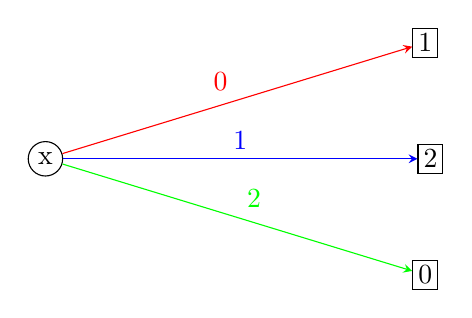
\begin{tikzpicture}[
node distance = 8pt and 64pt,
inner/.style={circle, draw=black, inner sep = 2pt, minimum size = 2pt},
terminal/.style={rectangle, draw=black, inner sep = 2pt, minimum size=2pt}]


\node[inner] (0c0) {x};
\node[terminal] (1) [above right = 32pt and 128pt of 0c0] {1};
\node[terminal] (2) [right = 128pt of 0c0] {2};
\node[terminal] (0) [below right = 32pt and 128pt of 0c0] {0};

\draw[-stealth, red] (0c0) to[edge label = 0] (1);
\draw[-stealth, blue] (0c0) to[edge label = 1] (2);
\draw[-stealth, green] (0c0) to[edge label = 2] (0);
\end{tikzpicture}
\end{center}
\end{example}

Using OMDDs it should be possible to generalize theorems $8$ and $9$ to an arbitrary prime $p$ in place of $2$ and an OMDD with every non-terminal node having out-degree $p$ with edges labeled by $0,\dots,p-1$ and with terminal nodes labeled by a subset of $\{0,\dots,p-1\}$ in place of BDDs.

For each $i \in \N$ let $p_i$ denote the $i$th largest prime. It follows from the Chinese remainder theorem that for every nonnegative integer $x$ if 
$$x \leq -1 + \prod_{i=1}^{n}p_i $$
then $x$ can be uniquely written in the form
$$\sum_{i=1}^{n} \left ( x_i \prod_{j \in \{1,\dots,n\}\setminus\{i\}}p_j \right ) - \gamma \prod_{j=1}^{n}p_j$$
where $\gamma \in \N_0$ and for each $i \in \{1,\dots,n\}$ $x_i \in \{0,\dots,p_i-1\}$. This is a special case of the \textit{residue numeral system}. Using the residue numeral system it should be possible to prove that the integer factorization problem for large enough $\alpha \in \N$ can represented as a small system of discrete functions with each function having a small OMDD representation, whereby `small' we mean bounded by a power of $\log(\alpha)$.

\subsection{Reduced boolean system}
For each $n \in \N_0$, let $g_n$ be the boolean function
$$\re_2 \left \qu_{2^{n}} \left (\re_{2^{n+1}}(-1-\alpha) + \sum_{k=1+u_n}^{n}2^{k}\sum_{j=0}^{k}x_jy_{k-j} \right ).$$
Using the orderings $<_n$ as defined in the previous section, if $u_{n+1}=u_n$ then using ordering $<_{n+1}$ for $g_n$ results in the same OBDD as constructed in the proof of Theorem $7$ and so typical OBDD manipulation algorithms give us an upper bound of the product of the sizes of the OBBDs for $g_n$ and $g_{n+1}$ for the OBDD $g_n g_{n+1}$, which in turn gives an upper bound of $\mathcal{O}(L_{\alpha}^6)$. If $u_{n+1} \neq u_n$ then $u_{n+1} = u_n+1$ and $<_n$ extended to include $y_{n+1}<y_n$ and $x_n<x_{n+1}$ can be transformed into $<_{n+1}$ or vice versa by $u_{n}+2$ transpositions, all of which are transpositions occuring between $x$ labels and $y$ labels within the $x,y$ alternating section of the order. Since in an OBDD transposition is a local operation any change in the number of nodes in the OBDD due to an order transposition will only change the number of nodes in the transposed levels. Since each level of each OBDD is at most $4(n+1)^2$, the number of nodes in the diagram increases by at most $c(n+1)^2$ where $c$ is a fixed positive integer. So the size of one of the OBDDs may increase by at most $(2+u_{n})c(n+1)^2 \leq c(n+2)(n+1)^2$, which means both diagrams are still cubic in $n$ and so their product will still be upper bounded by a constant times $L_{\alpha}^6$. This means it's possible to build an OBDD for the conjunction of the $g_n$s by way of starting with $g_N$, with $N = L_x+Ly+1$, then building an OBDD for $g_Ng_{N-1}$, then $g_{N}g_{N-1}g_{N-2}$, and so on, where at each step the size of the resulting product OBDD is bounded by the size of the previous product OBDD and $cL_{\alpha}^3$ for some fixed $c>0$. If the number of positive integers dividing $\alpha$ is small (e.g. $\alpha$ is the product of $2$ primes) then we also know that the conjunction of every OBDD in the system will be small. It is unknown how much expression swell will come into play.

For $p=2$, three other possible topics for future study are
\begin{enumerate}
\item Compare other normal form representations besides BDDs for the reduced system to the standard system.
\item Compare the performance of some CNF SAT solvers on CNF SAT instances obtained from the reduced system to those obtained from the standard system.
\item Look for further row reductions which can be applied to the reduced system.
\end{enumerate}

\newpage
\appendix
\section{Appendix}
In addition to Proposition 1, the derivations for the $p$-adic digit recurrences presented in section 3.2 use the following two facts. First, for each $N \in \N$ the restriction of $\qu_N$ to $\Z$ is increasing; therefore for all $N \in \N \setminus \{1\}$ and $x,y$ in the domain of $\re_N$ and $\qu_N$:
\begin{center}
\begin{array}{r c l}
0 \leq & \re_N(x)+\re_N(y)        & \leq N + N-2  \\
0 \leq & \qu_N(\re_N(x)+\re_N(y)) & \leq 1        \\
-(N-1) \leq & \re_N(x)-\re_N(y)   & \leq N-1 \\
-1 \leq & \qu_N(\re_N(x)- \re_N(y))  & \leq 0 \\
0 \leq & \re_N(x)\re_N(y)         & \leq N(N-2)+1 \\ 
0 \leq & \qu_N(\re_N(x)\re_N(y))  & \leq N-2 .
\end{array}
\end{center}
Second, if $R$ is a commutative ring with unity $1_R$ and additive identity $0_R$, $g : R \to R$, and $a \in \{0_R, 1_R\}$ then 
$$g(a) = (1_R-a)g(0_R) + a_Rg(1_R) = g(0_R) + (g(1_R) - g(0_R))a$$

\begin{itemize}
\item [Derivation for Addition:]
\begin{align*}
\qu_{p^n}(x+y) &= \qu_{p^n}(x)+\qu_{p^n}(y)+\qu_{p^n}(\re_{p^n}(x)+\re_{p^n}(y)) \\
\qu_{p^n}(\re_{p^n}(x)+\re_{p^n}(y)) &= \qu_{p}[\qu_{p^{n-1}}(\re_{p^n}(x)+\re_{p^n}(y))] \\
 &= \qu_{p}[ \qu_{p^{n-1}}(\re_{p^n}(x))+\qu_{p^{n-1}}(\re_{p^n}(y)) + 
\qu_{p^{n-1}}(\re_{p^{n-1}}(\re_{p^n}(x)) + \re_{p^{n-1}}(\re_{p^n}(y))) ] \\
&= \qu_{p}[ \re_p(\qu_{p^{n-1}}(x))+\re_p(\qu_{p^{n-1}}(y)) + 
\qu_{p^{n-1}}(\re_{p^{n-1}}(x) + \re_{p^{n-1}}(y)) ] \\
x_n &= \re_p(\qu_{p^n}(x)) \\
y_n &= \re_p(\qu_{p^n}(y)) \\
z_n &= \qu_{p^n}(\re_{p^n}(x)+\re_{p^n}(y)) \\
z_n &\in \{0,1\} \\
z_n &= \qu_p(x_{n-1}+y_{n-1}+z_{n-1}) \\
    &= (1-z_{n-1})\qu_p(x_{n-1}+y_{n-1}) + z_{n-1}\qu_p(x_{n-1}+y_{n-1}+1) \\
		&= \qu_p(x_{n-1}+y_{n-1}) +  z_{n-1}(\qu_p(x_{n-1}+y_{n-1}+1) - \qu_p(x_{n-1}+y_{n-1}) ) \\
		&= \qu_p(x_{n-1}+y_{n-1}) +  z_{n-1}\qu_p(\re_p(x_{n-1}+y_{n-1})+1).
\end{align*}

\item [Derivation for Subtraction:]
\begin{align*}
\qu_{p^n}(x-y) &= \qu_{p^n}(x)-\qu_{p^n}(y)+\qu_{p^n}(\re_{p^n}(x)-\re_{p^n}(y)) \\
\qu_{p^n}(\re_{p^n}(x)-\re_{p^n}(y)) &= \qu_{p}[\qu_{p^{n-1}}(\re_{p^n}(x)-\re_{p^n}(y))] \\
 &= \qu_{p}[ \qu_{p^{n-1}}(\re_{p^n}(x))-\qu_{p^{n-1}}(\re_{p^n}(y)) + 
\qu_{p^{n-1}}(\re_{p^{n-1}}(\re_{p^n}(x)) - \re_{p^{n-1}}(\re_{p^n}(y))) ] \\
&= \qu_{p}[ \re_p(\qu_{p^{n-1}}(x))-\re_p(\qu_{p^{n-1}}(y)) + 
\qu_{p^{n-1}}(\re_{p^{n-1}}(x) - \re_{p^{n-1}}(y)) ] \\
x_n &= \re_p(\qu_{p^n}(x)) \\
y_n &= \re_p(\qu_{p^n}(y)) \\
z_n &= \qu_{p^n}(\re_{p^n}(x)-\re_{p^n}(y)) \\
-z_n &\in \{0,1\} \\
z_n &= \qu_p(x_{n-1}-y_{n-1}-(-z_{n-1})) \\
    &= (1+z_{n-1})\qu_p(x_{n-1}-y_{n-1}) - z_{n-1}\qu_p(x_{n-1}-y_{n-1}-1) \\
		&= \qu_p(x_{n-1}-y_{n-1}) -  z_{n-1}(\qu_p(x_{n-1}-y_{n-1}-1) - \qu_p(x_{n-1}-y_{n-1}) ) \\
		&= \qu_p(x_{n-1}-y_{n-1}) -  z_{n-1}\qu_p(\re_p(x_{n-1}-y_{n-1})-1).
\end{align*}

\item [Derivation for Multiplication:]
\begin{align*}
a_{m,n} &= \qu_{p^m}(\re_{p^{n+1}}(x)y) \\
b_{m,n} &= \qu_{p^m}(x_ny) \\
c_{m,n} &= \qu_{p^m}(\re_{p^m}(\re_{p^n}(x)y) + \re_{p^m}(p^nx_ny)) \\
d_{m,n} &= \qu_{p}(\re_{p}(x_ny_m) + \qu_{p^{m}}(x_n\re_{p^{m}}(y))) \\
\qu_{p^n}(xy) &= \qu_{p^n}(x)y + \qu_{p^n}(\re_{p^n}(x)y) \\
              &= \qu_{p^n}(x)y + a_{n,n-1} \\
a_{m,n} &= \qu_{p^m}(\re_{p^{n+1}}(x)y) \\
        &= \qu_{p^m}((\re_{p^{n}}(x)+x_np^n)y) \\
				&= \qu_{p^m}(\re_{p^{n}}(x)y+x_np^ny) \\
				&= \qu_{p^m}(\re_{p^{n}}(x)y) + \qu_{p^m}(x_np^ny) + \qu_{p^m}(\re_{p^m}(\re_{p^{n}}(x)y)+\re_{p^m}(x_np^ny)) \\
				&= \qu_{p^m}(\re_{p^{n}}(x)y) + \qu_{p^{m-n}}(x_ny) + \qu_{p^m}(\re_{p^m}(\re_{p^{n}}(x)y)+\re_{p^m}(x_np^ny)) \\
				&= a_{m,n-1} + b_{m-n,n} + c_{m,n}.
\end{align*}
The recurrence for $c_{m,n}$ follows immediately from the derivation for the recurrence for addition. For $b_{m,n}$ we have
\begin{align*}
b_{m,n} &= \qu_{p^m}(x_ny) \\
        &= x_n\qu_{p^m}(y) + \qu_{p^m}(x_n\re_{p^m}(y)) \\
\qu_{p^m}(x_n\re_{p^m}(y)) &= \qu_{p}[\qu_{p^{m-1}}(x_n\re_{p^m}(y))] \\
        &= \qu_{p}[x_n\qu_{p^{m-1}}(\re_{p^m}(y)) + \qu_{p^{m-1}}(x_n\re_{p^{m-1}}(\re_{p^m}(y)))] \\
				&= \qu_{p}[x_n\re_p(\qu_{p^{m-1}}(y)) + \qu_{p^{m-1}}(x_n\re_{p^{m-1}}(y))] \\
				&= \qu_{p}[x_ny_{m-1} + \qu_{p^{m-1}}(x_n\re_{p^{m-1}}(y))] \\
				&= \qu_{p}(x_ny_{m-1}) + \qu_{p}[\re_p(x_ny_{m-1}) + \qu_{p^{m-1}}(x_n\re_{p^{m-1}}(y))] \\
				&= \qu_{p}(x_ny_{m-1}) + d_{m-1,n} \\
b_{m,n} &= x_n\qu_{p^m}(y) + \qu_{p}(x_ny_{m-1}) + d_{m-1,n}.
\end{align*}
Finally for $d_{m,n}$ note that $x_n\re_{p^m}(y) \leq (p-1)(p^{m}-1)$ and so $\qu_{p^m}(x_n\re_{p^{m}}(y)) \leq p-2$. Therefore it follows that $d_{m,n} \in \{0,1\}$ and so,
\begin{align*}
d_{m,n} &= \qu_{p}[\re_{p}(x_ny_m) + \qu_{p^{m}}(x_n\re_{p^{m}}(y))] \\
        &= \qu_{p}(\re_{p}(x_ny_m) + \qu_{p}(x_ny_{m-1}) + d_{m-1,n}) \\
				&= (1-d_{m-1,n})\qu_{p}(\re_{p}(x_ny_m) + \qu_{p}(x_ny_{m-1})) + d_{m,n}\qu_p(\re_{p}(x_ny_m) + \qu_{p}(x_ny_{m-1}) + 1) \\
				&= \qu_{p}(\re_{p}(x_ny_m) + \qu_{p}(x_ny_{m-1})) \\
				& \ \ + d_{m,n}[\qu_p(\re_{p}(x_ny_m) + \qu_{p}(x_ny_{m-1}) + 1) - \qu_{p}(\re_{p}(x_ny_m) + \qu_{p}(x_ny_{m-1}))] \\
				&= \qu_{p}(\re_{p}(x_ny_m) + \qu_{p}(x_ny_{m-1})) + d_{m,n}\qu_p(\re_{p}(x_ny_m + \qu_{p}(x_ny_{m-1})) + 1)
\end{align*}

\item [Derivation for Division:]
\begin{align*}
\frac{y}{x} &= \re_p\left ( \frac{y}{x} \right ) + p\frac{y-x\re_p\left ( \frac{y}{x} \right )}{px} \\
  &= \re_p\left ( \frac{y}{x} \right ) + p\frac{\qu_p \left ( y-x\re_p\left ( \frac{y}{x} \right ) \right )}{x} \\
	&= \re_p\left ( \frac{y}{x} \right ) + p\qu_p \left ( \frac{y}{x} \right ),\textrm{ and so} \\
\qu_p \left ( \frac{y}{x} \right ) &= \frac{\qu_p \left ( y-x\re_p\left ( \frac{y}{x} \right ) \right )}{x}.
\end{align*}
We use the preceding identity to derive the recurrence. For each $n \in \N_0$ let
$$d_n = x\qu_{p^n} \left ( \frac{y}{x} \right )$$
Then for $n > 0$
\begin{align*}
d_n &= x\qu_{p^n} \left ( \frac{y}{x} \right ) \\
    &= x\qu_p\left [ \qu_{p^{n-1}} \left ( \frac{y}{x} \right ) \right ]\\
		&= x\qu_p\left ( \frac{d_{n-1}}{x} \right ) \\
		&= x\qu_p\left ( \frac{d_{n-1}}{x} \right ) \\
		&= x\frac{\qu_p \left ( d_{n-1}-x\re_p\left ( \frac{d_{n-1}}{x} \right ) \right )}{x} \\
		&= \qu_p \left ( d_{n-1}-x\re_p\left ( \frac{d_{n-1}}{x} \right ) \right ) \\
		&= \qu_p \left ( d_{n-1} \right ) - \qu_p \left (x\re_p\left ( \frac{d_{n-1}}{x} \right ) \right ) + \qu_p \left ( \re_p(d_{n-1})-\re_p \left [ x\re_p\left ( \frac{d_{n-1}}{x} \right ) \right ] \right ) \\
		&= \qu_p \left ( d_{n-1} \right ) - \qu_p \left (x\re_p\left ( \frac{d_{n-1}}{x} \right ) \right ) + \qu_p \left ( \re_p(d_{n-1})-\re_p \left ( x\frac{d_{n-1}}{x} \right ) \right ) \\
		&= \qu_p \left ( d_{n-1} \right ) - \qu_p \left (x\re_p\left ( \frac{d_{n-1}}{x} \right ) \right ).
\end{align*}
For each $m,n \in \N_0$ let 
\begin{align*}
z_{m,n} &= \qu_{p^m}(d_n), \\
a_{m,n} &= \qu_{p^m}\left ( x \re_p \left ( \frac{z_{0,n}}{x_0} \right ) \right ), \\
b_{m,n} &= \qu_{p^m}(\re_{p^m}(z_{1,n}) - \re_{p^m}(a_{1,n})),\textrm{ and} \\
c_{m,n} &= \qu_p \left ( \re_p \left ( \frac{x_m z_{0,n}}{x_0} \right ) + \qu_{p^m} \left ( \re_{p^m}(x) \re_{p} \left [ \frac{z_{0,n}}{x_0} \right ] \right ) \right ).
\end{align*}
Then for $n>0$ the desired recurrences follow from the recurrences already derived for addition, subtraction, and multiplication. The recurrence for $a_{m,n}$ is derived in the same way as was done for the previous $b_{m,n}$ in the derivation for multiplication.
\end{itemize}

\newpage
\addcontentsline{toc}{section}{References}
\bibliography{thebib}
\bibliographystyle{ieeetr}
\end{document}